% Options for packages loaded elsewhere
\PassOptionsToPackage{unicode}{hyperref}
\PassOptionsToPackage{hyphens}{url}
%
\documentclass[
]{book}
\usepackage{amsmath,amssymb}
\usepackage{lmodern}
\usepackage{ifxetex,ifluatex}
\ifnum 0\ifxetex 1\fi\ifluatex 1\fi=0 % if pdftex
  \usepackage[T1]{fontenc}
  \usepackage[utf8]{inputenc}
  \usepackage{textcomp} % provide euro and other symbols
\else % if luatex or xetex
  \usepackage{unicode-math}
  \defaultfontfeatures{Scale=MatchLowercase}
  \defaultfontfeatures[\rmfamily]{Ligatures=TeX,Scale=1}
\fi
% Use upquote if available, for straight quotes in verbatim environments
\IfFileExists{upquote.sty}{\usepackage{upquote}}{}
\IfFileExists{microtype.sty}{% use microtype if available
  \usepackage[]{microtype}
  \UseMicrotypeSet[protrusion]{basicmath} % disable protrusion for tt fonts
}{}
\makeatletter
\@ifundefined{KOMAClassName}{% if non-KOMA class
  \IfFileExists{parskip.sty}{%
    \usepackage{parskip}
  }{% else
    \setlength{\parindent}{0pt}
    \setlength{\parskip}{6pt plus 2pt minus 1pt}}
}{% if KOMA class
  \KOMAoptions{parskip=half}}
\makeatother
\usepackage{xcolor}
\IfFileExists{xurl.sty}{\usepackage{xurl}}{} % add URL line breaks if available
\IfFileExists{bookmark.sty}{\usepackage{bookmark}}{\usepackage{hyperref}}
\hypersetup{
  pdftitle={PSC 253 Minimal Manual},
  pdfauthor={Matthew B. Platt},
  hidelinks,
  pdfcreator={LaTeX via pandoc}}
\urlstyle{same} % disable monospaced font for URLs
\usepackage{color}
\usepackage{fancyvrb}
\newcommand{\VerbBar}{|}
\newcommand{\VERB}{\Verb[commandchars=\\\{\}]}
\DefineVerbatimEnvironment{Highlighting}{Verbatim}{commandchars=\\\{\}}
% Add ',fontsize=\small' for more characters per line
\usepackage{framed}
\definecolor{shadecolor}{RGB}{248,248,248}
\newenvironment{Shaded}{\begin{snugshade}}{\end{snugshade}}
\newcommand{\AlertTok}[1]{\textcolor[rgb]{0.94,0.16,0.16}{#1}}
\newcommand{\AnnotationTok}[1]{\textcolor[rgb]{0.56,0.35,0.01}{\textbf{\textit{#1}}}}
\newcommand{\AttributeTok}[1]{\textcolor[rgb]{0.77,0.63,0.00}{#1}}
\newcommand{\BaseNTok}[1]{\textcolor[rgb]{0.00,0.00,0.81}{#1}}
\newcommand{\BuiltInTok}[1]{#1}
\newcommand{\CharTok}[1]{\textcolor[rgb]{0.31,0.60,0.02}{#1}}
\newcommand{\CommentTok}[1]{\textcolor[rgb]{0.56,0.35,0.01}{\textit{#1}}}
\newcommand{\CommentVarTok}[1]{\textcolor[rgb]{0.56,0.35,0.01}{\textbf{\textit{#1}}}}
\newcommand{\ConstantTok}[1]{\textcolor[rgb]{0.00,0.00,0.00}{#1}}
\newcommand{\ControlFlowTok}[1]{\textcolor[rgb]{0.13,0.29,0.53}{\textbf{#1}}}
\newcommand{\DataTypeTok}[1]{\textcolor[rgb]{0.13,0.29,0.53}{#1}}
\newcommand{\DecValTok}[1]{\textcolor[rgb]{0.00,0.00,0.81}{#1}}
\newcommand{\DocumentationTok}[1]{\textcolor[rgb]{0.56,0.35,0.01}{\textbf{\textit{#1}}}}
\newcommand{\ErrorTok}[1]{\textcolor[rgb]{0.64,0.00,0.00}{\textbf{#1}}}
\newcommand{\ExtensionTok}[1]{#1}
\newcommand{\FloatTok}[1]{\textcolor[rgb]{0.00,0.00,0.81}{#1}}
\newcommand{\FunctionTok}[1]{\textcolor[rgb]{0.00,0.00,0.00}{#1}}
\newcommand{\ImportTok}[1]{#1}
\newcommand{\InformationTok}[1]{\textcolor[rgb]{0.56,0.35,0.01}{\textbf{\textit{#1}}}}
\newcommand{\KeywordTok}[1]{\textcolor[rgb]{0.13,0.29,0.53}{\textbf{#1}}}
\newcommand{\NormalTok}[1]{#1}
\newcommand{\OperatorTok}[1]{\textcolor[rgb]{0.81,0.36,0.00}{\textbf{#1}}}
\newcommand{\OtherTok}[1]{\textcolor[rgb]{0.56,0.35,0.01}{#1}}
\newcommand{\PreprocessorTok}[1]{\textcolor[rgb]{0.56,0.35,0.01}{\textit{#1}}}
\newcommand{\RegionMarkerTok}[1]{#1}
\newcommand{\SpecialCharTok}[1]{\textcolor[rgb]{0.00,0.00,0.00}{#1}}
\newcommand{\SpecialStringTok}[1]{\textcolor[rgb]{0.31,0.60,0.02}{#1}}
\newcommand{\StringTok}[1]{\textcolor[rgb]{0.31,0.60,0.02}{#1}}
\newcommand{\VariableTok}[1]{\textcolor[rgb]{0.00,0.00,0.00}{#1}}
\newcommand{\VerbatimStringTok}[1]{\textcolor[rgb]{0.31,0.60,0.02}{#1}}
\newcommand{\WarningTok}[1]{\textcolor[rgb]{0.56,0.35,0.01}{\textbf{\textit{#1}}}}
\usepackage{longtable,booktabs,array}
\usepackage{calc} % for calculating minipage widths
% Correct order of tables after \paragraph or \subparagraph
\usepackage{etoolbox}
\makeatletter
\patchcmd\longtable{\par}{\if@noskipsec\mbox{}\fi\par}{}{}
\makeatother
% Allow footnotes in longtable head/foot
\IfFileExists{footnotehyper.sty}{\usepackage{footnotehyper}}{\usepackage{footnote}}
\makesavenoteenv{longtable}
\usepackage{graphicx}
\makeatletter
\def\maxwidth{\ifdim\Gin@nat@width>\linewidth\linewidth\else\Gin@nat@width\fi}
\def\maxheight{\ifdim\Gin@nat@height>\textheight\textheight\else\Gin@nat@height\fi}
\makeatother
% Scale images if necessary, so that they will not overflow the page
% margins by default, and it is still possible to overwrite the defaults
% using explicit options in \includegraphics[width, height, ...]{}
\setkeys{Gin}{width=\maxwidth,height=\maxheight,keepaspectratio}
% Set default figure placement to htbp
\makeatletter
\def\fps@figure{htbp}
\makeatother
\setlength{\emergencystretch}{3em} % prevent overfull lines
\providecommand{\tightlist}{%
  \setlength{\itemsep}{0pt}\setlength{\parskip}{0pt}}
\setcounter{secnumdepth}{5}
\usepackage{booktabs}
\usepackage{amsthm}
\makeatletter
\def\thm@space@setup{%
  \thm@preskip=8pt plus 2pt minus 4pt
  \thm@postskip=\thm@preskip
}
\makeatother
\ifluatex
  \usepackage{selnolig}  % disable illegal ligatures
\fi
\usepackage[]{natbib}
\bibliographystyle{plainnat}

\title{PSC 253 Minimal Manual}
\author{Matthew B. Platt}
\date{2021-08-20}

\begin{document}
\maketitle

{
\setcounter{tocdepth}{1}
\tableofcontents
}
\hypertarget{preface}{%
\chapter*{Preface}\label{preface}}
\addcontentsline{toc}{chapter}{Preface}

This book is a supplement to the book, \href{http://qss.princeton.press/}{Quantitative Social Science: An Introduction}, by Kosuke Imai. It also relies heavily on the work of \href{https://jrnold.github.io/qss-tidy/}{Jeffrey Arnold}, who translated the Imai code into tidyverse code.

I aspire for this text to act as a minimal manual for the course PSC 253 Scope and Methods in Political Science taught at Morehouse College. It is intended to cover all of the main analytical tasks that the course requires.

\hypertarget{basic}{%
\chapter{R Basics}\label{basic}}

At its most basic functionality, R is a calculator.

\hypertarget{calculate}{%
\section{Use R as a Calculator}\label{calculate}}

\hypertarget{problem}{%
\subsection{Problem}\label{problem}}

You want to add, subtract, multiply, divide, use exponents, and take square roots

\hypertarget{solution}{%
\subsection{Solution}\label{solution}}

Use \texttt{+} for addition, \texttt{-} for subtraction, \texttt{*} for multiplication and \texttt{/} for division.

\begin{Shaded}
\begin{Highlighting}[]
\CommentTok{\# addition}
\DecValTok{43} \SpecialCharTok{+} \DecValTok{5}
\end{Highlighting}
\end{Shaded}

\begin{verbatim}
## [1] 48
\end{verbatim}

\begin{Shaded}
\begin{Highlighting}[]
\CommentTok{\# subtraction}
\DecValTok{43} \SpecialCharTok{{-}} \DecValTok{5}
\end{Highlighting}
\end{Shaded}

\begin{verbatim}
## [1] 38
\end{verbatim}

\begin{Shaded}
\begin{Highlighting}[]
\CommentTok{\# multiplication}
\DecValTok{43} \SpecialCharTok{*} \DecValTok{5}
\end{Highlighting}
\end{Shaded}

\begin{verbatim}
## [1] 215
\end{verbatim}

\begin{Shaded}
\begin{Highlighting}[]
\CommentTok{\# division}
\DecValTok{43}\SpecialCharTok{/}\DecValTok{5}
\end{Highlighting}
\end{Shaded}

\begin{verbatim}
## [1] 8.6
\end{verbatim}

For exponents, we raise \texttt{X} to the power of \texttt{y} by using \texttt{\^{}}. That is \texttt{X\^{}y}.

\begin{Shaded}
\begin{Highlighting}[]
\CommentTok{\# raise 43 to the power of 5}
\DecValTok{43} \SpecialCharTok{\^{}} \DecValTok{5}
\end{Highlighting}
\end{Shaded}

\begin{verbatim}
## [1] 147008443
\end{verbatim}

Take the square root of some number \texttt{x} by using the function \texttt{sqrt()}. That is \texttt{sqrt(x)}.

\begin{Shaded}
\begin{Highlighting}[]
\CommentTok{\# take the square root of 43}
\FunctionTok{sqrt}\NormalTok{(}\DecValTok{43}\NormalTok{)}
\end{Highlighting}
\end{Shaded}

\begin{verbatim}
## [1] 6.557439
\end{verbatim}

\hypertarget{troubleshooting}{%
\subsection{Troubleshooting}\label{troubleshooting}}

\begin{itemize}
\tightlist
\item
  Keep in mind that R follows the order of operations, 2 + 2 * 2 is equal to 6 and not 8.
\end{itemize}

\begin{Shaded}
\begin{Highlighting}[]
\CommentTok{\# correct}
\DecValTok{2} \SpecialCharTok{+} \DecValTok{2} \SpecialCharTok{*} \DecValTok{2}
\end{Highlighting}
\end{Shaded}

\begin{verbatim}
## [1] 6
\end{verbatim}

\begin{Shaded}
\begin{Highlighting}[]
\CommentTok{\# incorrect}
\NormalTok{(}\DecValTok{2} \SpecialCharTok{+} \DecValTok{2}\NormalTok{) }\SpecialCharTok{*} \DecValTok{2}
\end{Highlighting}
\end{Shaded}

\begin{verbatim}
## [1] 8
\end{verbatim}

\hypertarget{object}{%
\section{Creating an Object}\label{object}}

\hypertarget{problem-1}{%
\subsection{Problem}\label{problem-1}}

You want to create an object to hold a number

\hypertarget{solution-1}{%
\subsection{Solution}\label{solution-1}}

To create an object:

\begin{enumerate}
\def\labelenumi{\arabic{enumi}.}
\tightlist
\item
  type in a name for the object, like \texttt{newobject} then
\item
  use the assignment operator \texttt{\textless{}-},
\item
  input a number, mathematical expression, dataset, or text on the right side of \texttt{\textless{}-} that you want assigned to the \texttt{newobject}
\end{enumerate}

\begin{Shaded}
\begin{Highlighting}[]
\CommentTok{\# assigning the number 4 to a new object named "myobject"}
\NormalTok{myobject }\OtherTok{\textless{}{-}} \DecValTok{4}

\CommentTok{\# assigning the text "hallelujah hollaback" to a new object named "second\_object"}
\NormalTok{second\_object }\OtherTok{\textless{}{-}} \StringTok{"hallelujah hollaback"}
\end{Highlighting}
\end{Shaded}

Type the name of an object in order to see what it contains.

\begin{Shaded}
\begin{Highlighting}[]
\NormalTok{myobject}
\end{Highlighting}
\end{Shaded}

\begin{verbatim}
## [1] 4
\end{verbatim}

\begin{Shaded}
\begin{Highlighting}[]
\NormalTok{second\_object}
\end{Highlighting}
\end{Shaded}

\begin{verbatim}
## [1] "hallelujah hollaback"
\end{verbatim}

\hypertarget{troubleshooting-1}{%
\subsection{Troubleshooting}\label{troubleshooting-1}}

\begin{itemize}
\tightlist
\item
  There cannot be any spaces in the name of an object. Instead you could use dots, dashes, underscores, or capitalization to distinguish between words: \texttt{small.data}, \texttt{big-data}, \texttt{bigger\_data}, \texttt{mediumData}.
\item
  Text needs to be in quotation marks in order to be assigned to an object.
\item
  Object names are case sensitive \texttt{Myobject} is not the same as \texttt{myobject}
\end{itemize}

\hypertarget{vector}{%
\section{Creating a Vector}\label{vector}}

A vector is a list of numbers or characters. We will create vectors for a variety of reasons in this course.

\hypertarget{problem-2}{%
\subsection{Problem}\label{problem-2}}

You want to create a vector.

\hypertarget{solution-2}{%
\subsection{Solution}\label{solution-2}}

Use the function \texttt{c()} to create a list by separating the entries with a comma.

\begin{Shaded}
\begin{Highlighting}[]
\CommentTok{\# create a vector called \textquotesingle{}prime\textquotesingle{}}
\NormalTok{prime }\OtherTok{\textless{}{-}} \FunctionTok{c}\NormalTok{(}\DecValTok{1}\NormalTok{, }\DecValTok{3}\NormalTok{, }\DecValTok{5}\NormalTok{, }\DecValTok{7}\NormalTok{)}

\NormalTok{prime}
\end{Highlighting}
\end{Shaded}

\begin{verbatim}
## [1] 1 3 5 7
\end{verbatim}

\begin{Shaded}
\begin{Highlighting}[]
\CommentTok{\# create a vector called "first\_name"}
\NormalTok{first\_name }\OtherTok{\textless{}{-}} \FunctionTok{c}\NormalTok{(}\StringTok{"Matthew"}\NormalTok{, }\StringTok{"Mosi"}\NormalTok{, }\StringTok{"Manu"}\NormalTok{, }\StringTok{"Ekundayo"}\NormalTok{, }\StringTok{"Kwasi"}\NormalTok{)}

\NormalTok{first\_name}
\end{Highlighting}
\end{Shaded}

\begin{verbatim}
## [1] "Matthew"  "Mosi"     "Manu"     "Ekundayo" "Kwasi"
\end{verbatim}

\hypertarget{troubleshooting-2}{%
\subsection{Troubleshooting}\label{troubleshooting-2}}

\begin{itemize}
\tightlist
\item
  As the name of a function, \texttt{c()} is case sensitive. Use the lowercase \texttt{c}.
\item
  Make sure that all elements are separated by a comma.
\item
  Vectors are typically assigned to some object.
\end{itemize}

\hypertarget{index}{%
\section{Indexing}\label{index}}

We can use indexing to pull out specific sets of observations from a vector or dataset.

\hypertarget{problem-3}{%
\subsection{Problem}\label{problem-3}}

You want to select a specific one observation based on its position within a vector or matrix.

\hypertarget{solution-3}{%
\subsection{Solution}\label{solution-3}}

We index by using the brackets \texttt{{[}x,\ y{]}} after an object where x is the row and y is the column.

\begin{Shaded}
\begin{Highlighting}[]
\CommentTok{\# we have a vector}
\NormalTok{prime }\OtherTok{\textless{}{-}} \FunctionTok{c}\NormalTok{(}\DecValTok{1}\NormalTok{, }\DecValTok{3}\NormalTok{, }\DecValTok{5}\NormalTok{, }\DecValTok{7}\NormalTok{)}

\CommentTok{\# we want the number 3, which is the second observation in the vector}
\NormalTok{prime[}\DecValTok{2}\NormalTok{]}
\end{Highlighting}
\end{Shaded}

\begin{verbatim}
## [1] 3
\end{verbatim}

\begin{Shaded}
\begin{Highlighting}[]
\CommentTok{\# we have a matrix}
\NormalTok{yup }\OtherTok{\textless{}{-}} \FunctionTok{matrix}\NormalTok{(}\FunctionTok{c}\NormalTok{(prime,}\DecValTok{2}\NormalTok{, }\DecValTok{6}\NormalTok{, }\DecValTok{10}\NormalTok{, }\DecValTok{14}\NormalTok{), }\AttributeTok{nrow =} \DecValTok{2}\NormalTok{, }\AttributeTok{ncol =} \DecValTok{4}\NormalTok{, }\AttributeTok{byrow =}\NormalTok{ T)}
\NormalTok{yup}
\end{Highlighting}
\end{Shaded}

\begin{verbatim}
##      [,1] [,2] [,3] [,4]
## [1,]    1    3    5    7
## [2,]    2    6   10   14
\end{verbatim}

\begin{Shaded}
\begin{Highlighting}[]
\CommentTok{\# We want the observation in the first row and fourth column}
\NormalTok{yup[}\DecValTok{1}\NormalTok{, }\DecValTok{4}\NormalTok{]}
\end{Highlighting}
\end{Shaded}

\begin{verbatim}
## [1] 7
\end{verbatim}

\hypertarget{problem-4}{%
\subsection{Problem}\label{problem-4}}

You want to select an entire row or column.

\hypertarget{solution-4}{%
\subsection{Solution}\label{solution-4}}

You can select an entire row by leaving the column index position blank \texttt{yup{[}2,\ {]}}. You can select an entire column by leaving the row index position blank \texttt{yup{[}\ ,\ 2{]}}.

\begin{Shaded}
\begin{Highlighting}[]
\CommentTok{\# We have our matrix}
\NormalTok{yup}
\end{Highlighting}
\end{Shaded}

\begin{verbatim}
##      [,1] [,2] [,3] [,4]
## [1,]    1    3    5    7
## [2,]    2    6   10   14
\end{verbatim}

\begin{Shaded}
\begin{Highlighting}[]
\CommentTok{\# We want the second row}
\NormalTok{yup[}\DecValTok{1}\NormalTok{, ]}
\end{Highlighting}
\end{Shaded}

\begin{verbatim}
## [1] 1 3 5 7
\end{verbatim}

\begin{Shaded}
\begin{Highlighting}[]
\CommentTok{\# We want the third column}
\NormalTok{yup[ , }\DecValTok{3}\NormalTok{]}
\end{Highlighting}
\end{Shaded}

\begin{verbatim}
## [1]  5 10
\end{verbatim}

\hypertarget{project}{%
\section{Creating a Project}\label{project}}

Creating a project creates a folder on your computer that Rstudio and R will treat as the default directory for your code. That is, whenever you tell R to look for something on your computer, it will begin by looking in the project folder.

\hypertarget{problem-5}{%
\subsection{Problem}\label{problem-5}}

You want to create a new project.

\hypertarget{solution-5}{%
\subsection{Solution}\label{solution-5}}

There are multiple ways to create a new project. You can go to the menu bar and select ``File'', then ``New Project'':

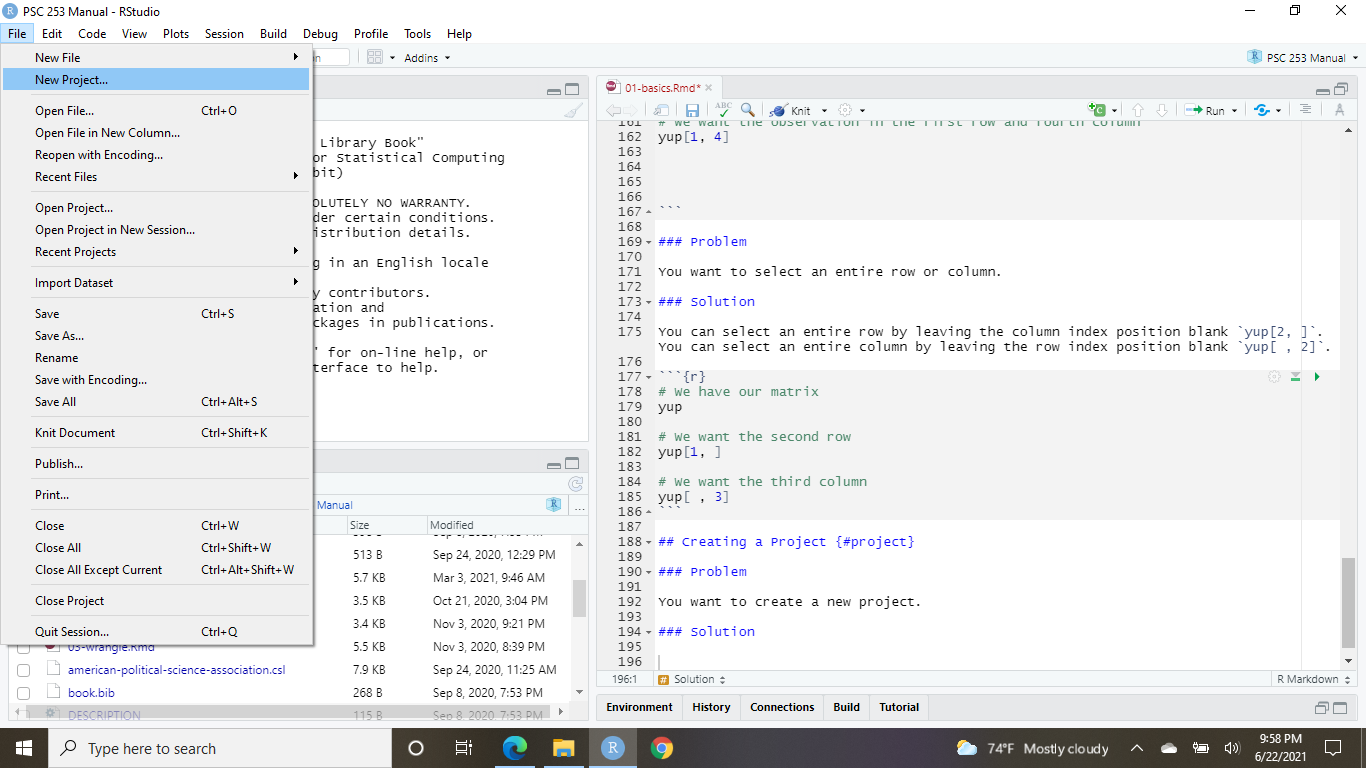
\includegraphics[width=18.97in]{images/projectfile}

You can click the ``create project'' icon on the toolbar:

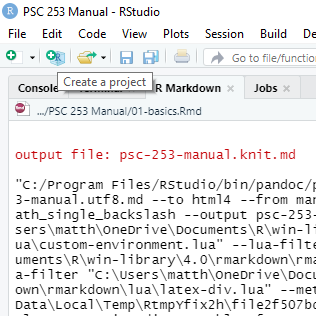
\includegraphics[width=4.39in]{images/projectbar}

Or you can select ``New Project'' from the project menu at the top left of Rstudio:

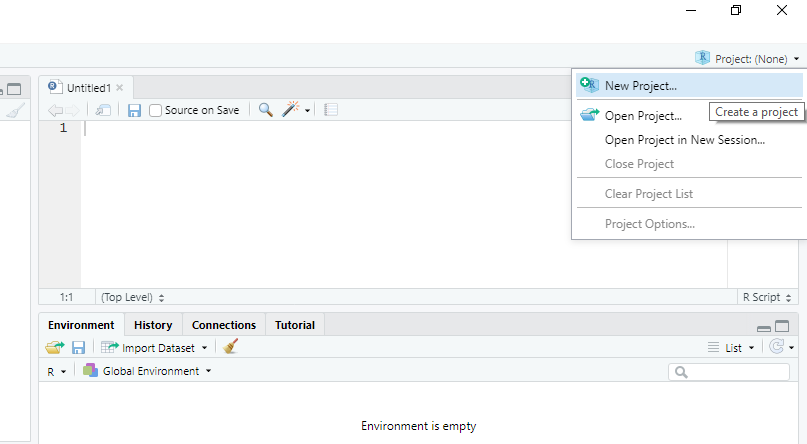
\includegraphics[width=11.21in]{images/projectmenu}

When you select ``New Project'', the below dialogue box appears. Select ``New Directory'':

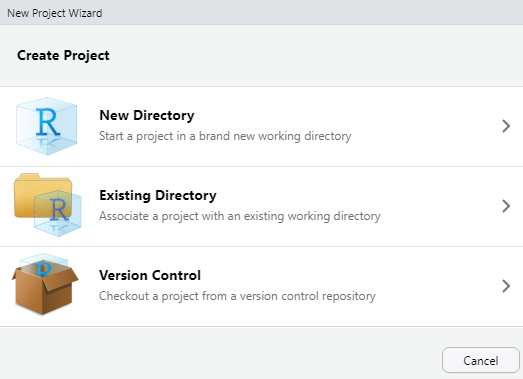
\includegraphics[width=7.26in]{images/projoption1}

Then select ``New project'',

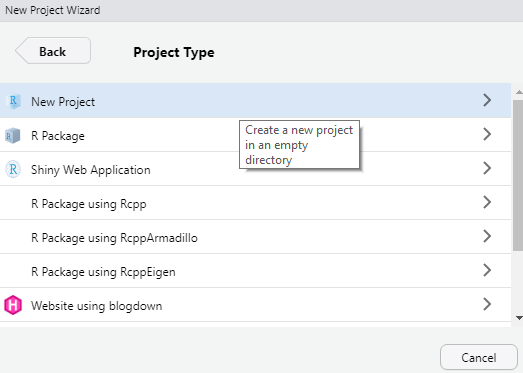
\includegraphics[width=7.26in]{images/projoption2}

enter a name for the project, and browse to where you want the directory located on your computer.

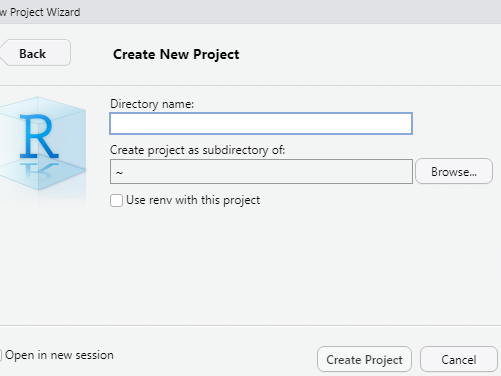
\includegraphics[width=6.96in]{images/projdirectory}

Complete the process by clicking ``Create Project.''

\hypertarget{troubleshooting-3}{%
\subsection{Troubleshooting}\label{troubleshooting-3}}

\begin{itemize}
\tightlist
\item
  You need to know where your project folders are on your computer. I recommend that you create a master folder called ``PSC 253'', and then have all of your project folders inside of that master folder.
\item
  We will use separate projects for each lab assignment and for the Data Project assignment.
\item
  Avoid having multiple project folders for the same assignment. It will cause confusion when you are trying to submit the correct project folder for your assignment.
\end{itemize}

\hypertarget{installpack}{%
\section{Installing a Package}\label{installpack}}

A \emph{package} is a specialized collection of R elements -- datasets, functions, objects, etc. We will use various packages to help in our data analysis. Packages have to be installed and loaded before their elements can be accessed, so this section will teach you how to install a package.

\hypertarget{problem-6}{%
\subsection{Problem}\label{problem-6}}

You want to install a package.

\hypertarget{solution-6}{%
\subsection{Solution}\label{solution-6}}

\begin{enumerate}
\def\labelenumi{\arabic{enumi}.}
\tightlist
\item
  You can type in the command \texttt{install.packages("packagename")}. Thus, to install the package named ``here'' we would type \texttt{install.packages("here")}.
\end{enumerate}

\begin{Shaded}
\begin{Highlighting}[]
\CommentTok{\# installing the poliscidata package}

\FunctionTok{install.packages}\NormalTok{(}\StringTok{"poliscidata"}\NormalTok{)}
\end{Highlighting}
\end{Shaded}

Alternatively, you can use the menu bar:

\begin{enumerate}
\def\labelenumi{\arabic{enumi}.}
\tightlist
\item
  Click on ``Tools'' in the menu bar.
\item
  select ``Install Packages''
\item
  A dialogue box will appear.
\item
  Type in the name of the package you want.
\item
  Click ``Install''.
\end{enumerate}

\hypertarget{troubleshooting-4}{%
\subsection{Troubleshooting}\label{troubleshooting-4}}

\begin{itemize}
\tightlist
\item
  Some packages depend on the installation of other packages first. R will install these dependencies automatically, so it may take a while for your package to install. You know the installation is done when the console shows its arrow and blinking cursor.
\item
  If you get a message asking you to install Rtools, then you can do so {[}here{]}{[}\url{https://cran.r-project.org/bin/windows/Rtools/}{]}.
\item
  If you get a message that says ``exited with non-zero status'', then the package did not fully install. This could be due to one of the dependency packages not installing properly. Try to install that dependency package manually -- \texttt{install.packages("dependencyname")}. Once the dependent package is installed, you can try to install the main package again.
\item
  You will know that the package has been successfully installed if you are able to load the package.
\item
  In rare occasions, a package may require a later edition of R than you have installed on your computer. The message will say something like ``This package requires R 4.1.0 and you have R 3.1.0''. In that case, you will need to download and install the latest version of R before you can install the package.
\item
  Remember to use quotation marks around the package name in \texttt{install.packages()}.
\end{itemize}

\hypertarget{loadpack}{%
\section{Loading a Package}\label{loadpack}}

It is not enough to just install a package. Installed packages must be loaded in order for you to access their elements.

\hypertarget{problem-7}{%
\subsection{Problem}\label{problem-7}}

You want to load a package that you have installed.

\hypertarget{solution-7}{%
\subsection{Solution}\label{solution-7}}

The function we use to load packages is \texttt{library()}. Its main argument is the name of the package -- \texttt{library(packagename)}.

\begin{Shaded}
\begin{Highlighting}[]
\CommentTok{\# load the poliscidata package}

\FunctionTok{library}\NormalTok{(poliscidata)}
\end{Highlighting}
\end{Shaded}

\hypertarget{troubleshooting-5}{%
\subsection{Troubleshooting}\label{troubleshooting-5}}

\begin{itemize}
\tightlist
\item
  Packages must be fully and properly installed before they can be loaded.
\item
  If you get an error saying that a package does not exist then 1) you have not installed the package or 2) you have spelled the name of the package incorrectly.
\item
  Remember that we do not put the name of the package in quotation marks when we are loading it.
\end{itemize}

\hypertarget{relative-path}{%
\section{Using relative file paths}\label{relative-path}}

Whenever we load data or save data we will need to specify a file path -- where the file is located on the computer. Obviously, the file path on your computer will not be the same as the path on someone else's computer. We want our code to be able to run on any computer, so we create \emph{relative} file paths. That is, we specify where the file is located relative to the \protect\hyperlink{project}{project folder}.

\hypertarget{problem-8}{%
\subsection{Problem}\label{problem-8}}

You want to create a file path relative to the project folder.

\hypertarget{solution-8}{%
\subsection{Solution}\label{solution-8}}

\begin{enumerate}
\def\labelenumi{\arabic{enumi}.}
\tightlist
\item
  You need to already have a project folder. See Section \ref{project}.
\item
  Load the ``here'' package
\item
  The function \texttt{here()} automatically sets the relative point of the file path as the location of your \texttt{.Rproj} file.
\item
  You can then provide the file path as the argument to \texttt{here()}.
\end{enumerate}

\begin{Shaded}
\begin{Highlighting}[]
\CommentTok{\# Creating a path to the "images" folder in this project.}

\FunctionTok{library}\NormalTok{(here)}
\end{Highlighting}
\end{Shaded}

\begin{verbatim}
## here() starts at E:/OneDrive/R Code/PSC 253 Manual
\end{verbatim}

\begin{Shaded}
\begin{Highlighting}[]
\FunctionTok{here}\NormalTok{(}\StringTok{"images"}\NormalTok{)}
\end{Highlighting}
\end{Shaded}

\begin{verbatim}
## [1] "E:/OneDrive/R Code/PSC 253 Manual/images"
\end{verbatim}

For example, we have a project folder named ``hypothesis\_test\_lab''. Figure \ref{fig:here-example} shows the inside of that project folder. There are three subfolders: Data, Documents, and Scripts. Inside the ``Data'' folder there are two more folders called \texttt{Analysis\_Data} and \texttt{Original\_Data}.

\textbackslash begin\{figure\}
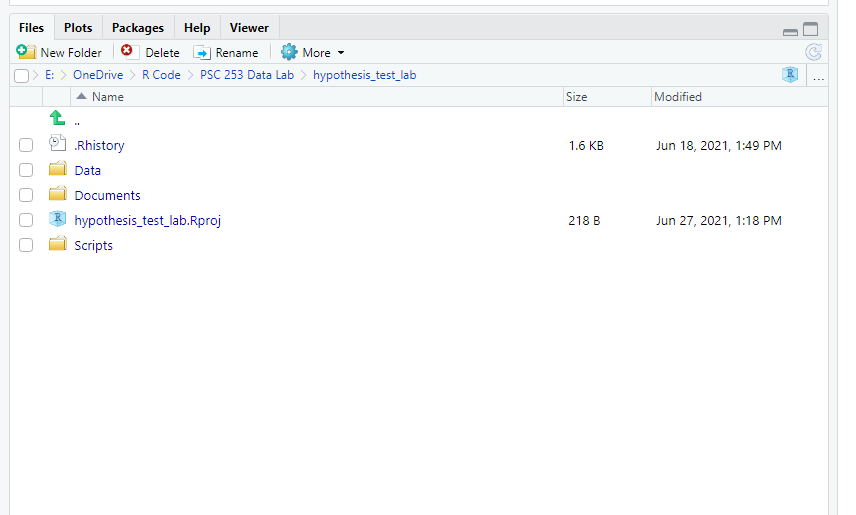
\includegraphics[width=11.89in]{images/here_example1} \textbackslash caption\{A screen shot of the hypothesis\_test\_lab project folder.\}\label{fig:here-example}
\textbackslash end\{figure\}

We will use the \texttt{here()} function to load a data file that is found within the \texttt{Analysis\_Data} folder.

\begin{Shaded}
\begin{Highlighting}[]
\CommentTok{\# loading "analysis1.RData" file}

\FunctionTok{load}\NormalTok{(}\FunctionTok{here}\NormalTok{(}\StringTok{"Data/Analysis\_Data/analysis1.RData"}\NormalTok{))}
\end{Highlighting}
\end{Shaded}

\hypertarget{troubleshooting-6}{%
\subsection{Troubleshooting}\label{troubleshooting-6}}

\begin{itemize}
\tightlist
\item
  Remember to use forward slashes \texttt{/} and quotation marks when writing the relative path for \texttt{here()}.
\item
  The use of \texttt{here()} is a new function introduced in Fall 2021. Code from prior versions of the course that used relative paths may need to be revised if you want to use the \texttt{here()} function.
\item
  Your first code chunk should load the \texttt{here} package -- \texttt{library(here)}.
\end{itemize}

\hypertarget{csv-load}{%
\section{Loading .csv Data}\label{csv-load}}

There are some packages that come with datasets attached to them. However, we will mostly need to import datasets into R. This section deals with how to specify the file path for the data and the various functions that correspond to the different types of data files you may encounter.

\hypertarget{problem-9}{%
\subsection{Problem}\label{problem-9}}

You want to load a datafile that takes the form \texttt{data\_name.csv}.

\hypertarget{solution-9}{%
\subsection{Solution}\label{solution-9}}

\begin{enumerate}
\def\labelenumi{\arabic{enumi}.}
\tightlist
\item
  You already have a project folder. (Section \ref{project})
\item
  You already know how to create relative paths. (Section \ref{relative-path})
\item
  In this course, \texttt{.csv} files should always be located in the \texttt{Original\_Data} subfolder, which is found inside the ``Data'' folder.
\item
  \protect\hyperlink{object}{Create an object} to hold the data that you will import. This object will be assigned the imported data.
\item
  Use the function \texttt{read.csv()} or \texttt{read\_csv()} to import the data into R. Its argument is the file path.
\end{enumerate}

Generically, the code takes the form:

\begin{Shaded}
\begin{Highlighting}[]
\NormalTok{your\_object }\OtherTok{\textless{}{-}} \FunctionTok{read.csv}\NormalTok{(}\FunctionTok{here}\NormalTok{(}\StringTok{"Data/Original\_Data/your\_data.csv"}\NormalTok{))}
\end{Highlighting}
\end{Shaded}

If I were loading a csv file named ``congbills.csv'' and assigning it to an object called ``bills'', then the code would be:

\begin{Shaded}
\begin{Highlighting}[]
\CommentTok{\# Loading the csv file "congbills.csv" into R as an object called "bills"}

\NormalTok{bills }\OtherTok{\textless{}{-}} \FunctionTok{read.csv}\NormalTok{(}\FunctionTok{here}\NormalTok{(}\StringTok{"Data/Original\_Data/congbills.csv"}\NormalTok{))}
\end{Highlighting}
\end{Shaded}

\hypertarget{troubleshooting-7}{%
\subsection{Troubleshooting}\label{troubleshooting-7}}

\begin{itemize}
\tightlist
\item
  The most common error is that the file path to the data has not been specified properly. Check the spelling in your file path.
\item
  Make sure that you use \texttt{here()} for the file path. Start from the project folder, and then write the path until you get to your file.
\item
  Using \texttt{read\_csv()} requires the \texttt{tidyverse} package.
\end{itemize}

\hypertarget{dta-load}{%
\section{Loading .dta Data}\label{dta-load}}

Stata is another popular software program for data analysis. It is often used in economics. The types of files that are used in Stata have the suffix \texttt{.dta}.

\hypertarget{problem-10}{%
\subsection{Problem}\label{problem-10}}

You want to load a datafile that takes the form \texttt{data\_name.dta}.

\hypertarget{solution-10}{%
\subsection{Solution}\label{solution-10}}

\begin{enumerate}
\def\labelenumi{\arabic{enumi}.}
\tightlist
\item
  You already have a project folder. (Section \ref{project})
\item
  You already know how to create relative paths. (Section \ref{relative-path})
\item
  In this course, \texttt{.dta} files should always be located in the \texttt{Original\_Data} subfolder, which is found inside the ``Data'' folder.
\item
  \protect\hyperlink{object}{Create an object} to hold the data that you will import. This object will be assigned the imported data.
\item
  \protect\hyperlink{loadpack}{Load the package} \texttt{haven} -- \texttt{library(haven)}
\item
  Use the function \texttt{read\_dta()} to import the data into R. Its argument is the file path.
\end{enumerate}

Generically, the code takes the form:

\begin{Shaded}
\begin{Highlighting}[]
\CommentTok{\# load the package \textquotesingle{}haven\textquotesingle{}}
\FunctionTok{library}\NormalTok{(haven)}

\CommentTok{\# import the data}
\NormalTok{your\_object }\OtherTok{\textless{}{-}} \FunctionTok{read\_data}\NormalTok{(}\FunctionTok{here}\NormalTok{(}\StringTok{"Data/Original\_Data/your\_data.dta"}\NormalTok{))}
\end{Highlighting}
\end{Shaded}

If I were loading a dta file named ``congbills.dta'' and assigning it to an object called ``bills'', then the code would be:

\begin{Shaded}
\begin{Highlighting}[]
\CommentTok{\# Loading the csv file "congbills.csv" into R as an object called "bills"}

\NormalTok{bills }\OtherTok{\textless{}{-}} \FunctionTok{read\_dta}\NormalTok{(}\FunctionTok{here}\NormalTok{(}\StringTok{"Data/Original\_Data/congbills.dta"}\NormalTok{))}
\end{Highlighting}
\end{Shaded}

\hypertarget{troubleshooting-8}{%
\subsection{Troubleshooting}\label{troubleshooting-8}}

\begin{itemize}
\tightlist
\item
  The most common error is that the file path to the data has not been specified properly. Check the spelling in your file path.
\item
  Make sure that you use \texttt{here()} for the file path. Start from the project folder, and then write the path until you get to your file.
\item
  Using \texttt{read\_dta()} requires the \texttt{haven} package.
\end{itemize}

\hypertarget{bivariate-comparisons}{%
\chapter{Bivariate Comparisons}\label{bivariate-comparisons}}

\hypertarget{crosstab}{%
\section{Crosstab}\label{crosstab}}

\hypertarget{problem-11}{%
\subsection{Problem}\label{problem-11}}

You want to make a crosstab.

\hypertarget{solution-11}{%
\subsection{Solution}\label{solution-11}}

\begin{enumerate}
\def\labelenumi{\arabic{enumi}.}
\tightlist
\item
  Load the \texttt{poliscidata} package.
\item
  In order to create a crosstab in R, we use the function called \texttt{xtp()}.\\
\item
  The function follows the following template:
\end{enumerate}

\begin{Shaded}
\begin{Highlighting}[]
\FunctionTok{xtp}\NormalTok{(}\AttributeTok{data =}\NormalTok{ your data, }\AttributeTok{y =}\NormalTok{ dependent variable, }\AttributeTok{x =}\NormalTok{ independent variable, }\AttributeTok{w =}\NormalTok{ weights)}
\end{Highlighting}
\end{Shaded}

\begin{enumerate}
\def\labelenumi{\arabic{enumi}.}
\tightlist
\item
  Specify the dataset, the dependent variable, the independent variable, and the weights (if applicable)
\end{enumerate}

\begin{Shaded}
\begin{Highlighting}[]
\CommentTok{\# Create a crosstab where the dependent variable is "envjob\_3", the independent variable is "pid\_3", and the weights are "wt".}
\CommentTok{\# The dataset is "nes", which is found in the "poliscidata" package.}
\FunctionTok{xtp}\NormalTok{(}\AttributeTok{data =}\NormalTok{ nes, }\AttributeTok{y =}\NormalTok{ envjob\_3, }\AttributeTok{x =}\NormalTok{ pid\_3, }\AttributeTok{w =}\NormalTok{ wt)}
\end{Highlighting}
\end{Shaded}

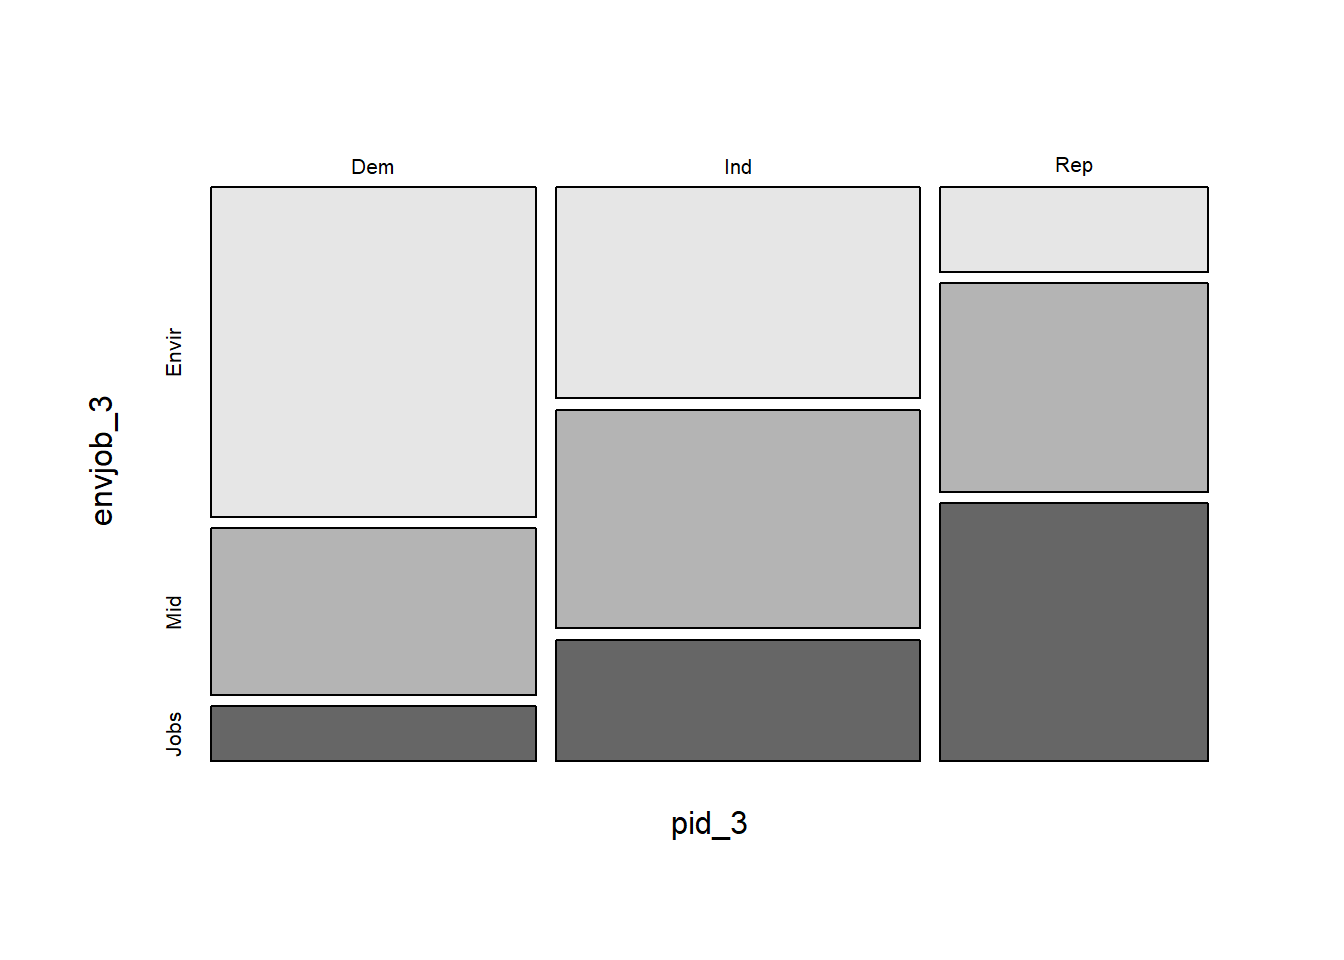
\includegraphics{psc-253-manual_files/figure-latex/unnamed-chunk-26-1.pdf}

\begin{verbatim}
##    Cell Contents 
## |-------------------------|
## |                   Count | 
## |          Column Percent | 
## |-------------------------|
## 
## ============================================
##             pid_3
## envjob_3       Dem      Ind      Rep   Total
## --------------------------------------------
## Envir        1005      721      212    1938 
##             59.82%   38.25%   15.30%        
## --------------------------------------------
## Mid           508      749      525    1782 
##             30.24%   39.73%   37.88%        
## --------------------------------------------
## Jobs          167      415      649    1231 
##              9.94%   22.02%   46.83%        
## --------------------------------------------
## Total        1680     1885     1386    4951 
##             33.93%   38.07%   27.99%        
## ============================================
\end{verbatim}

\hypertarget{troubleshooting-9}{%
\subsection{Troubleshooting}\label{troubleshooting-9}}

\begin{itemize}
\tightlist
\item
  Make sure that the \texttt{poliscidata} package is loaded. Use \texttt{library(poliscidata)} to load.
\item
  The arguments for the independent and dependent variables are just the variable names. They do not follow the template of \texttt{data\$variable}.
\item
  Crosstabs are used when both the independent and dependent variables are categorical. Avoid making a crosstab with numeric data.
\end{itemize}

\hypertarget{compmeans}{%
\section{Comparison of Means}\label{compmeans}}

\hypertarget{problem-12}{%
\subsection{Problem}\label{problem-12}}

You want to make a comparison of means table.

\hypertarget{solution-12}{%
\subsection{Solution}\label{solution-12}}

\begin{enumerate}
\def\labelenumi{\arabic{enumi}.}
\tightlist
\item
  Load the \texttt{poliscidata} package.
\item
  In order to create a comparison of means table in R, we use the function called \texttt{compmeans()}.\\
\item
  The function follows the following template:
\end{enumerate}

\begin{Shaded}
\begin{Highlighting}[]
\FunctionTok{compmeans}\NormalTok{(}\AttributeTok{x =}\NormalTok{ data}\SpecialCharTok{$}\NormalTok{dependent, }\AttributeTok{f =}\NormalTok{ data}\SpecialCharTok{$}\NormalTok{independent)}
\end{Highlighting}
\end{Shaded}

Here is a comparison of means table for feelings towards Obama \texttt{obama\_therm} by party identification \texttt{pid\_x}.

\begin{Shaded}
\begin{Highlighting}[]
\CommentTok{\# create the comparison of means table}
\FunctionTok{compmeans}\NormalTok{(}\AttributeTok{x =}\NormalTok{ nes}\SpecialCharTok{$}\NormalTok{obama\_therm, }\AttributeTok{f =}\NormalTok{ nes}\SpecialCharTok{$}\NormalTok{pid\_x, }
          \AttributeTok{weights =}\NormalTok{ nes}\SpecialCharTok{$}\NormalTok{wt)}
\end{Highlighting}
\end{Shaded}

\begin{verbatim}
## Warning in descr::compmeans(...): 442 rows with missing values dropped
\end{verbatim}

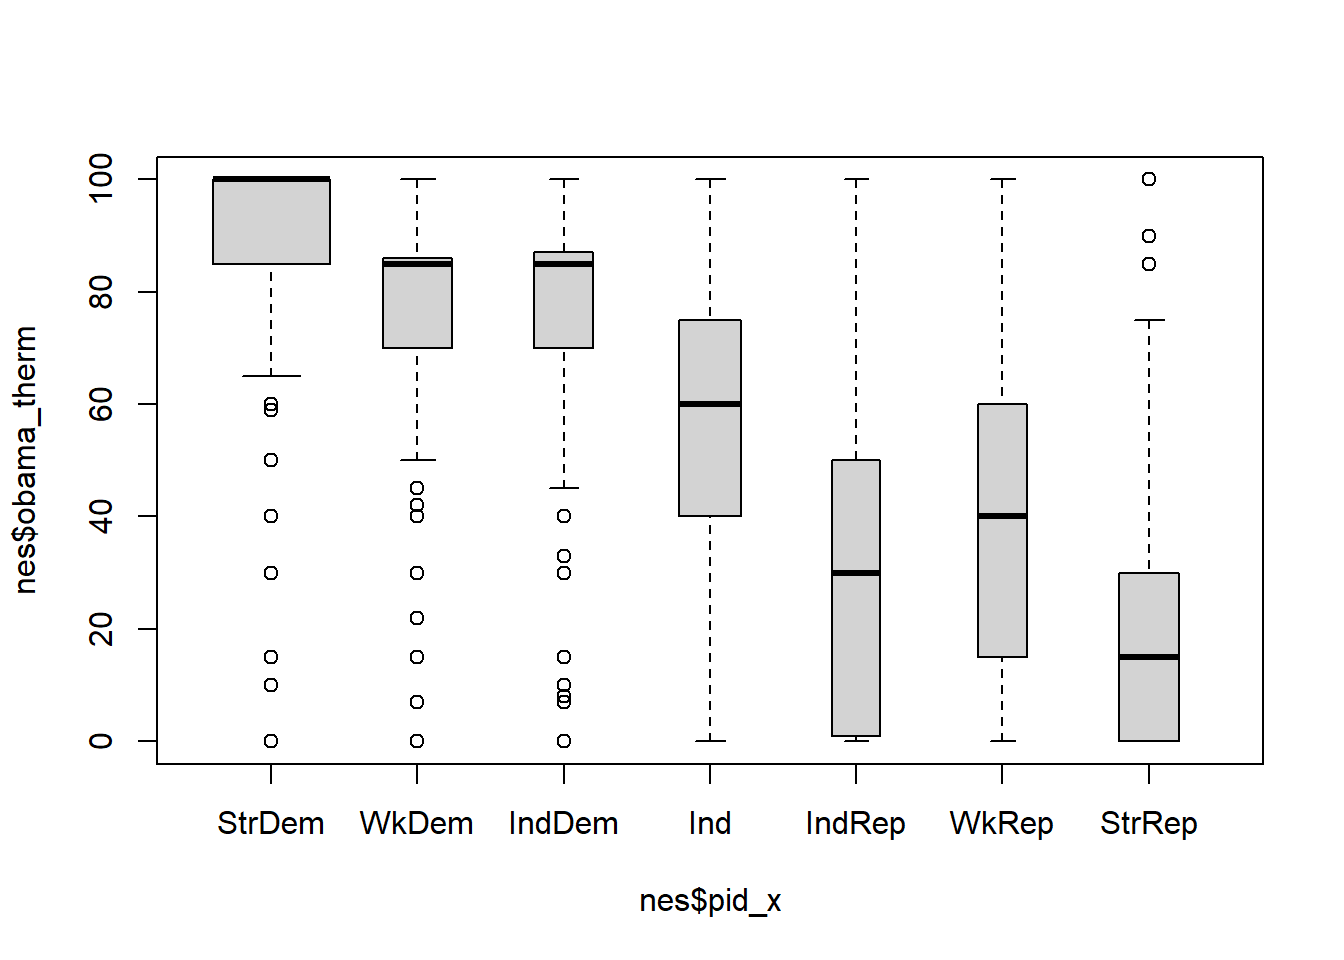
\includegraphics{psc-253-manual_files/figure-latex/unnamed-chunk-28-1.pdf}

\begin{verbatim}
## Mean value of "nes$obama_therm" according to "nes$pid_x"
##            Mean    N Std. Dev.
## StrDem 91.12934 1384  14.19526
## WkDem  75.39237  813  22.08436
## IndDem 76.11223  695  20.22679
## Ind    54.56354  724  29.85396
## IndRep 32.15929  565  27.71165
## WkRep  36.67241  580  27.85999
## StrRep 18.44039  713  22.65842
## Total  60.72470 5474  34.64432
\end{verbatim}

\hypertarget{troubleshooting-10}{%
\subsection{Troubleshooting}\label{troubleshooting-10}}

\begin{itemize}
\tightlist
\item
  Make sure \texttt{poliscidata} is loaded.
\item
  Keep in mind that the variables follow the pattern of \texttt{data\$variable}.
\item
  You only need to specify the weights argument if you have survey data with survey weights.
\end{itemize}

\hypertarget{barchart}{%
\section{Make a Bar Chart}\label{barchart}}

\hypertarget{problem-13}{%
\subsection{Problem}\label{problem-13}}

Make a barchart that plots the mean of a dependent variable (Y) by an independent variable (X).

\hypertarget{solution-13}{%
\subsection{Solution}\label{solution-13}}

\begin{enumerate}
\def\labelenumi{\arabic{enumi}.}
\tightlist
\item
  Create a summary dataset to plot (see \ref{sum}).
\item
  Use \texttt{ggplot()} for the data and the mapping.
\item
  The data is the summary dataset, \texttt{data\ =\ sum\_data}
\item
  The mapping is \texttt{mapping\ =\ aes(x\ =\ independent,\ y\ =\ dependent)}
\item
  If you want to color the bars, add \texttt{fill\ =\ independent} to the mapping.
\item
  Use a \texttt{+} at the end of the line of code.
\item
  Use \texttt{geom\_col()} to make the bar shapes.
\end{enumerate}

\begin{Shaded}
\begin{Highlighting}[]
\NormalTok{p1 }\OtherTok{\textless{}{-}} \FunctionTok{ggplot}\NormalTok{(}\AttributeTok{data =}\NormalTok{ sum\_data, }
             \AttributeTok{mapping =} \FunctionTok{aes}\NormalTok{(}\AttributeTok{x =}\NormalTok{ independent, }\AttributeTok{y =}\NormalTok{ dependent)) }\SpecialCharTok{+}
  \FunctionTok{geom\_col}\NormalTok{()}
\end{Highlighting}
\end{Shaded}

Plot the mean feelings towards Obama \texttt{obama\_therm} by party identification \texttt{pid\_x}.

\begin{Shaded}
\begin{Highlighting}[]
\CommentTok{\# create the summary dataset}
\NormalTok{partymeans }\OtherTok{\textless{}{-}}\NormalTok{ nes }\SpecialCharTok{\%\textgreater{}\%}
  \FunctionTok{group\_by}\NormalTok{(pid\_x) }\SpecialCharTok{\%\textgreater{}\%}
  \FunctionTok{summarise}\NormalTok{(}\AttributeTok{average =} \FunctionTok{wtd.mean}\NormalTok{(obama\_therm, }\AttributeTok{na.rm =}\NormalTok{ T,}
                               \AttributeTok{weights =}\NormalTok{ wt))}

\CommentTok{\# specify the data and mapping}
\NormalTok{p1 }\OtherTok{\textless{}{-}} \FunctionTok{ggplot}\NormalTok{(}\AttributeTok{data =}\NormalTok{ partymeans,}
             \AttributeTok{mapping =} \FunctionTok{aes}\NormalTok{(}\AttributeTok{x =}\NormalTok{ pid\_x, }\AttributeTok{y =}\NormalTok{ average)) }\SpecialCharTok{+}
  
  \CommentTok{\# add the bar shape}
  \FunctionTok{geom\_col}\NormalTok{()}

\CommentTok{\# print the plot}
\NormalTok{p1}
\end{Highlighting}
\end{Shaded}

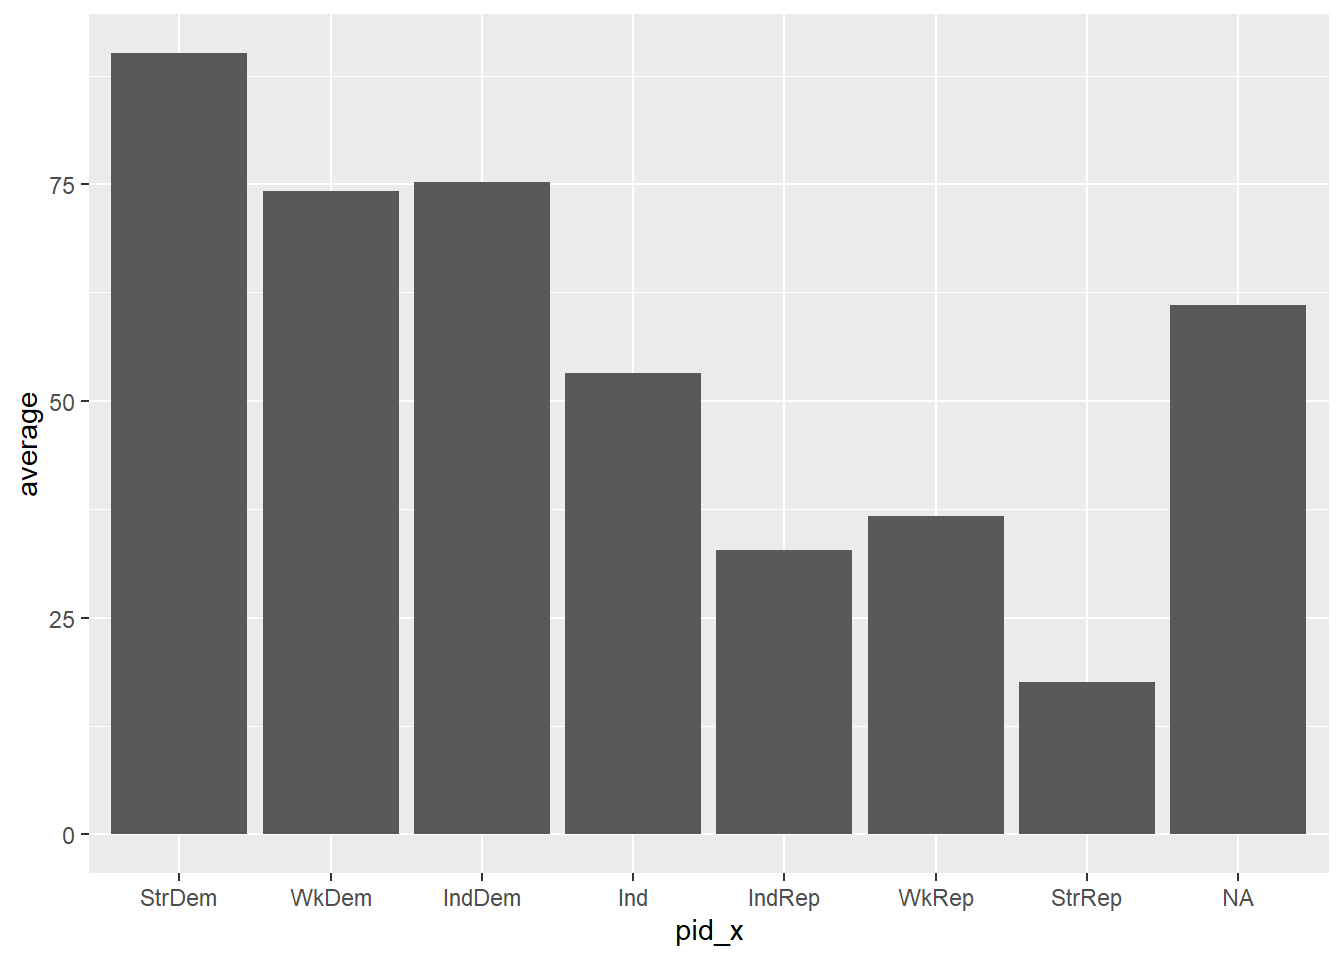
\includegraphics{psc-253-manual_files/figure-latex/unnamed-chunk-30-1.pdf}

\hypertarget{troubleshooting-11}{%
\subsection{Troubleshooting}\label{troubleshooting-11}}

\begin{itemize}
\tightlist
\item
  Make sure that you use the summary dataset instead of the larger dataset.
\item
  If there are errors in making the summary dataset, then there will be problems in the plot.
\item
  You need to load the \texttt{tidyverse} package.
\end{itemize}

\hypertarget{data-wrangling}{%
\chapter{Data Wrangling}\label{data-wrangling}}

\hypertarget{factor}{%
\section{Create a Factor Variable}\label{factor}}

\hypertarget{problem-14}{%
\subsection{Problem}\label{problem-14}}

You want to transform a variable into a factor.

\hypertarget{solution-14}{%
\subsection{Solution}\label{solution-14}}

\begin{enumerate}
\def\labelenumi{\arabic{enumi}.}
\tightlist
\item
  Decide on what to name the factor variable.
\item
  Use \texttt{as.factor()} to assign the old variable values to the new variable.
\item
  Use \texttt{levels()} to assign labels to the values of the variable.
\item
  The levels should be provided as a list in \texttt{c()} with the names of the levels in quotation marks.
\item
  It would follow the general template below.
\end{enumerate}

\begin{Shaded}
\begin{Highlighting}[]
\CommentTok{\# define the variable as a factor}

\NormalTok{data}\SpecialCharTok{$}\NormalTok{newvariable }\OtherTok{\textless{}{-}} \FunctionTok{as.factor}\NormalTok{(data}\SpecialCharTok{$}\NormalTok{oldvariable)}

\CommentTok{\# add the levels}

\FunctionTok{levels}\NormalTok{(data}\SpecialCharTok{$}\NormalTok{newvariable) }\OtherTok{\textless{}{-}} \FunctionTok{c}\NormalTok{(}\StringTok{"label1"}\NormalTok{, }\StringTok{"label2"}\NormalTok{, }\StringTok{"labelk"}\NormalTok{)}
\end{Highlighting}
\end{Shaded}

Transform \texttt{obama\_vote} in the \texttt{nes} from a numeric dummy variable into a factor.

\begin{Shaded}
\begin{Highlighting}[]
\CommentTok{\# the frequency table for the old variable}
\FunctionTok{freq}\NormalTok{(nes}\SpecialCharTok{$}\NormalTok{obama\_vote)}
\end{Highlighting}
\end{Shaded}

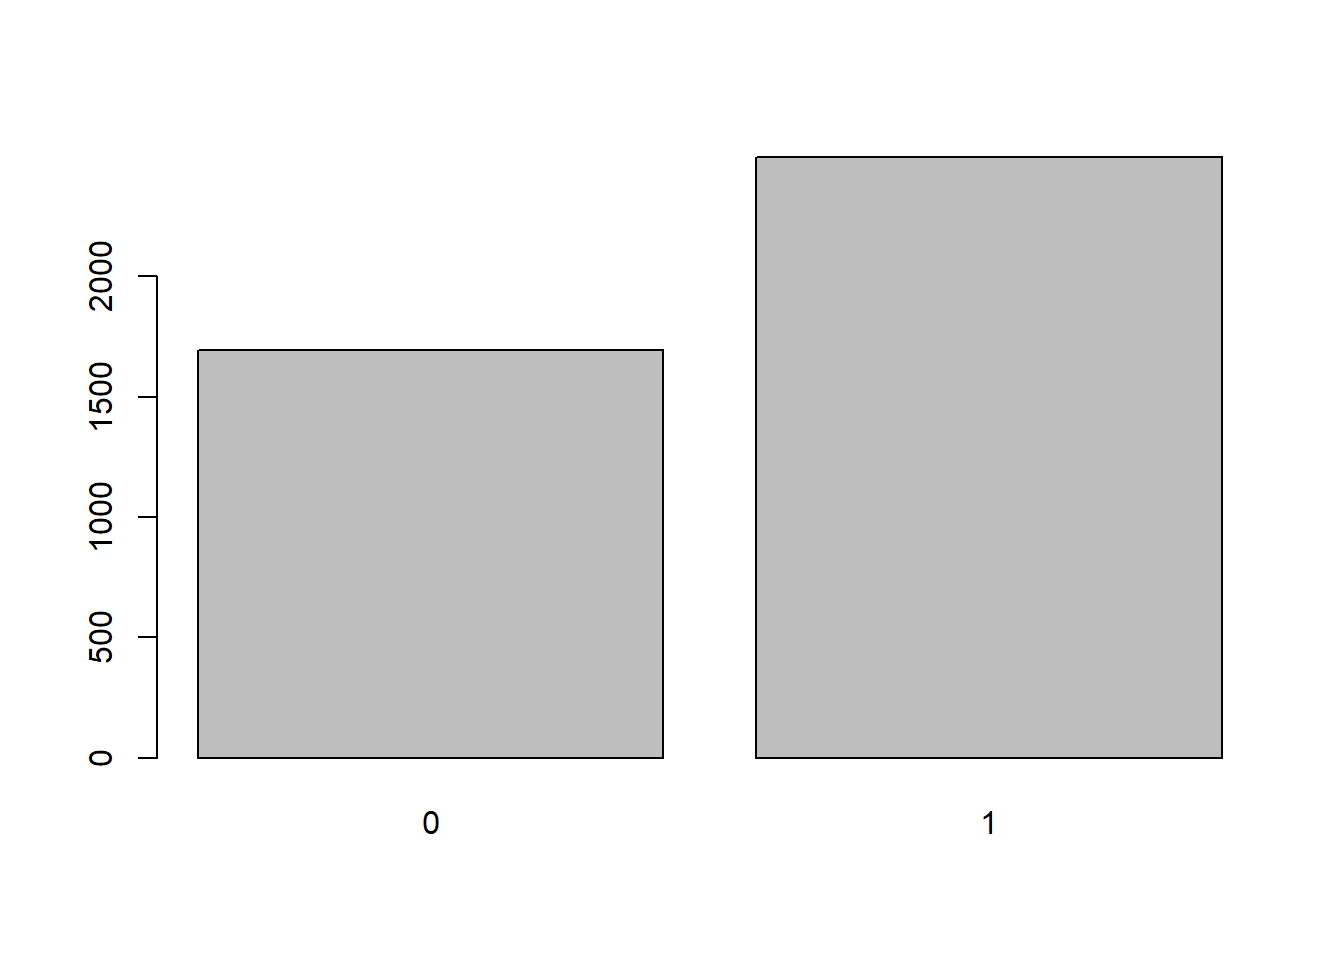
\includegraphics{psc-253-manual_files/figure-latex/unnamed-chunk-32-1.pdf}

\begin{verbatim}
## nes$obama_vote 
##       Frequency Percent Valid Percent
## 0          1692   28.60          40.4
## 1          2496   42.19          59.6
## NA's       1728   29.21              
## Total      5916  100.00         100.0
\end{verbatim}

\begin{Shaded}
\begin{Highlighting}[]
\CommentTok{\# call the new variable \textasciigrave{}obamafct\textasciigrave{}}
\NormalTok{nes}\SpecialCharTok{$}\NormalTok{obamafct }\OtherTok{\textless{}{-}} \FunctionTok{as.factor}\NormalTok{(nes}\SpecialCharTok{$}\NormalTok{obama\_vote)}

\CommentTok{\# assign the levels}
\FunctionTok{levels}\NormalTok{(nes}\SpecialCharTok{$}\NormalTok{obamafct) }\OtherTok{\textless{}{-}} \FunctionTok{c}\NormalTok{(}\StringTok{"did not vote for Obama"}\NormalTok{, }\StringTok{"voted for Obama"}\NormalTok{)}

\CommentTok{\# the frequency table for the new variable}
\FunctionTok{freq}\NormalTok{(nes}\SpecialCharTok{$}\NormalTok{obamafct)}
\end{Highlighting}
\end{Shaded}

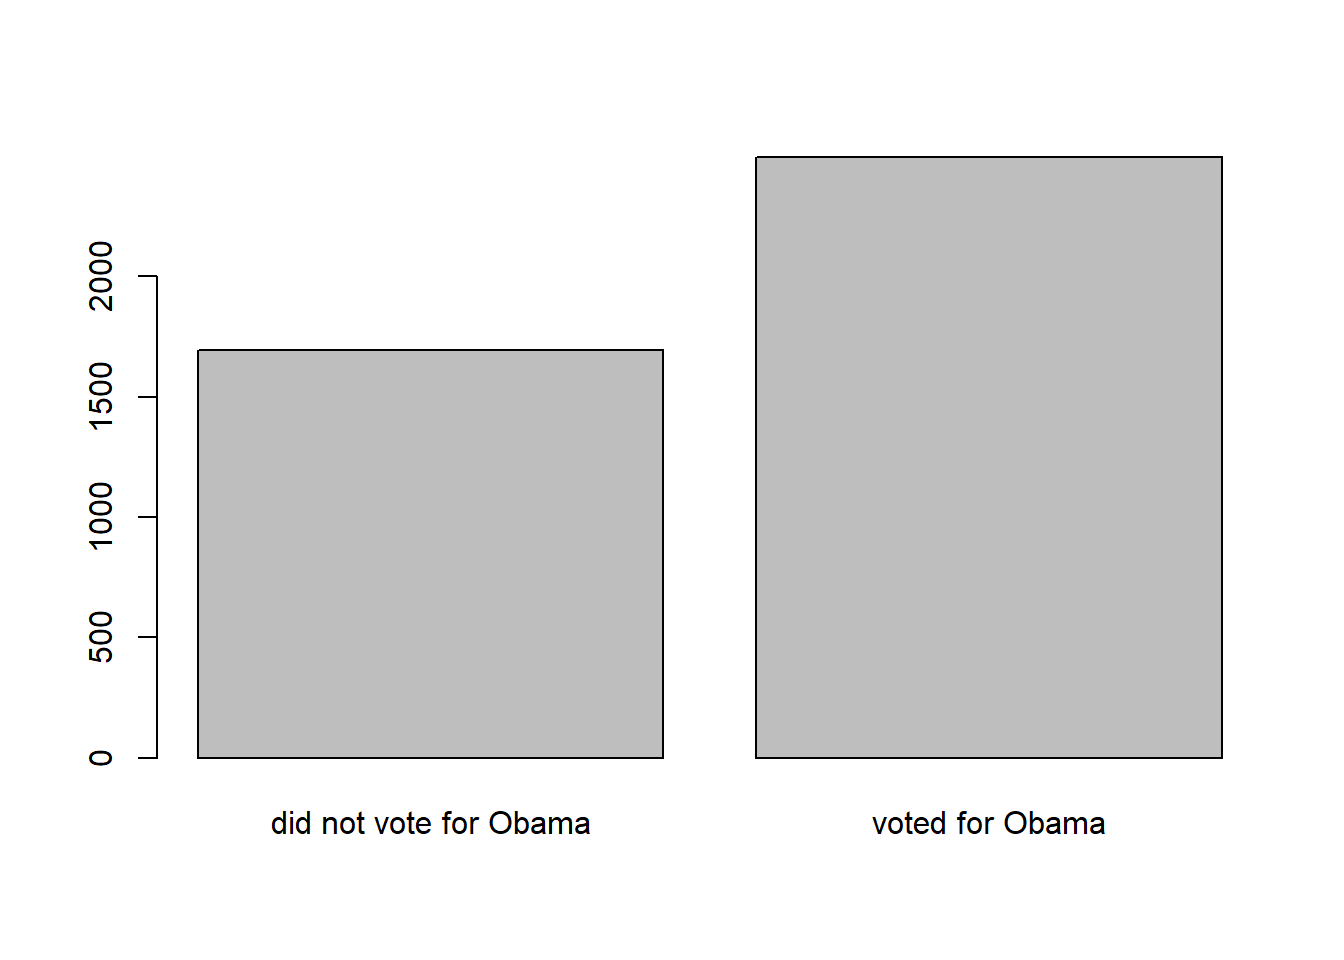
\includegraphics{psc-253-manual_files/figure-latex/unnamed-chunk-32-2.pdf}

\begin{verbatim}
## nes$obamafct 
##                        Frequency Percent Valid Percent
## did not vote for Obama      1692   28.60          40.4
## voted for Obama             2496   42.19          59.6
## NA's                        1728   29.21              
## Total                       5916  100.00         100.0
\end{verbatim}

\hypertarget{troubleshooting-12}{%
\subsection{Troubleshooting}\label{troubleshooting-12}}

\begin{itemize}
\item
  There has to be a level provided for each value of the variable. That is why this process should occur after a variable has been cleaned.
\item
  The level names do not have to be unique. That means this could be used as a (somewhat clunky) method of recoding a variable by collapsing its categories.
\end{itemize}

\hypertarget{numeric}{%
\section{Create a Numeric Variable}\label{numeric}}

\hypertarget{problem-15}{%
\subsection{Problem}\label{problem-15}}

You want to transform an existing variable into a numeric variable.

\hypertarget{solution-15}{%
\subsection{Solution}\label{solution-15}}

\begin{enumerate}
\def\labelenumi{\arabic{enumi}.}
\tightlist
\item
  Decide on what to name the numeric variable. It could be the same name as the old variable.
\item
  Use \texttt{as.numeric()} to assign the old variable values to the new variable.
\item
  It would follow the general template below.
\end{enumerate}

\begin{Shaded}
\begin{Highlighting}[]
\NormalTok{data}\SpecialCharTok{$}\NormalTok{newvariable }\OtherTok{\textless{}{-}} \FunctionTok{as.numeric}\NormalTok{(data}\SpecialCharTok{$}\NormalTok{oldvariable)}
\end{Highlighting}
\end{Shaded}

Here is an example that converts the seven-point party identification scale into a numeric variable.

\begin{Shaded}
\begin{Highlighting}[]
\CommentTok{\# frequency table of the original variable \textasciigrave{}pid\_x\textasciigrave{}}
\FunctionTok{freq}\NormalTok{(nes}\SpecialCharTok{$}\NormalTok{pid\_x)}
\end{Highlighting}
\end{Shaded}

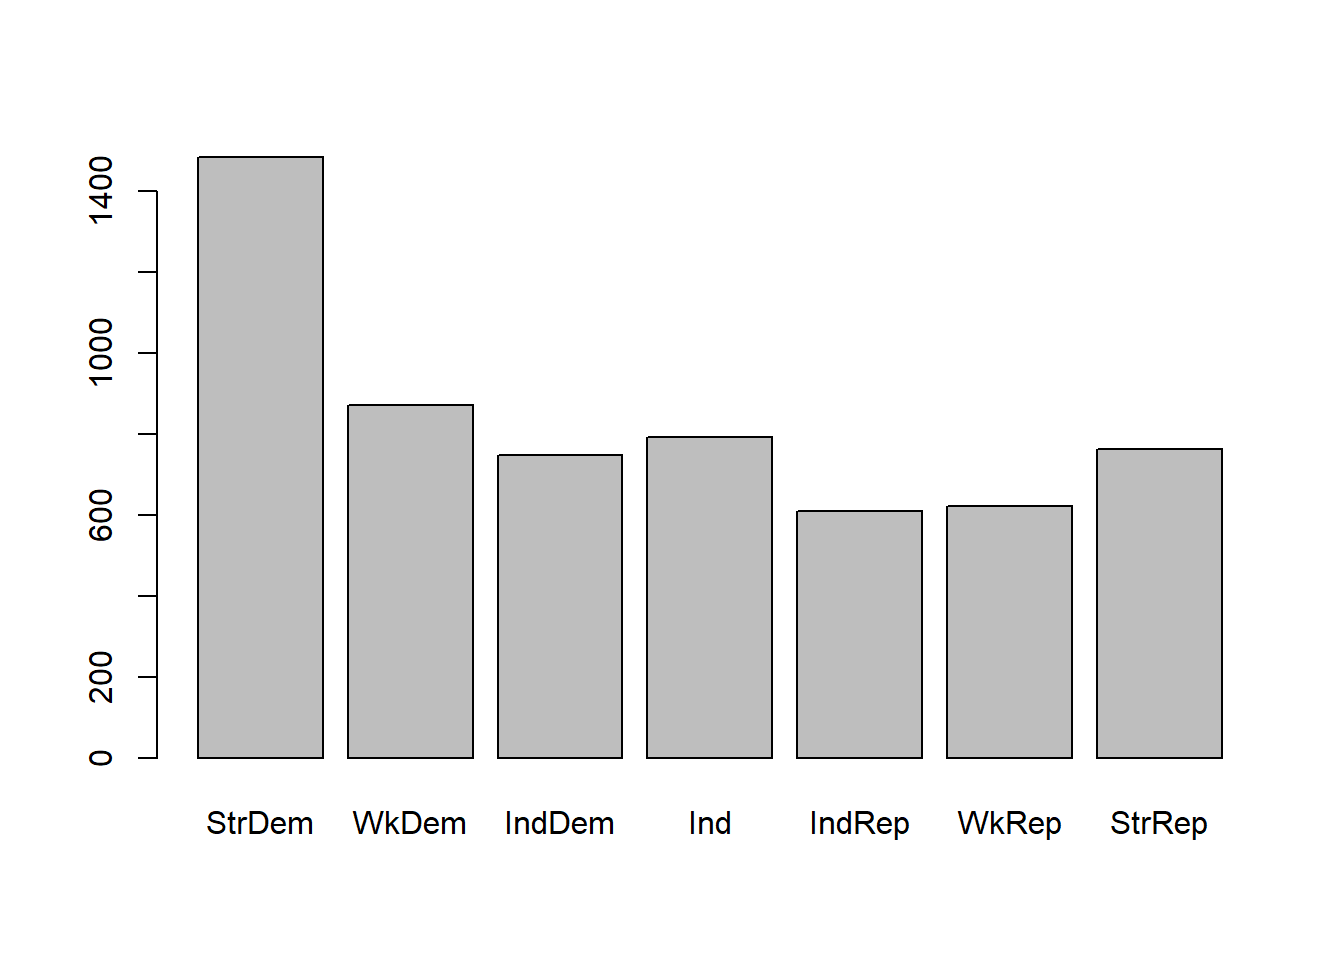
\includegraphics{psc-253-manual_files/figure-latex/unnamed-chunk-34-1.pdf}

\begin{verbatim}
## nes$pid_x 
##        Frequency  Percent Valid Percent
## StrDem      1485  25.1014         25.20
## WkDem        873  14.7566         14.82
## IndDem       747  12.6268         12.68
## Ind          792  13.3874         13.44
## IndRep       610  10.3110         10.35
## WkRep        623  10.5308         10.57
## StrRep       762  12.8803         12.93
## NA's          24   0.4057              
## Total       5916 100.0000        100.00
\end{verbatim}

\begin{Shaded}
\begin{Highlighting}[]
\CommentTok{\# make \textasciigrave{}pid\_x\textasciigrave{} numeric}
\NormalTok{nes}\SpecialCharTok{$}\NormalTok{pid7 }\OtherTok{\textless{}{-}} \FunctionTok{as.numeric}\NormalTok{(nes}\SpecialCharTok{$}\NormalTok{pid\_x)}

\CommentTok{\# frequency table of the new variable \textasciigrave{}pid7\textasciigrave{}}
\FunctionTok{freq}\NormalTok{(nes}\SpecialCharTok{$}\NormalTok{pid7)}
\end{Highlighting}
\end{Shaded}

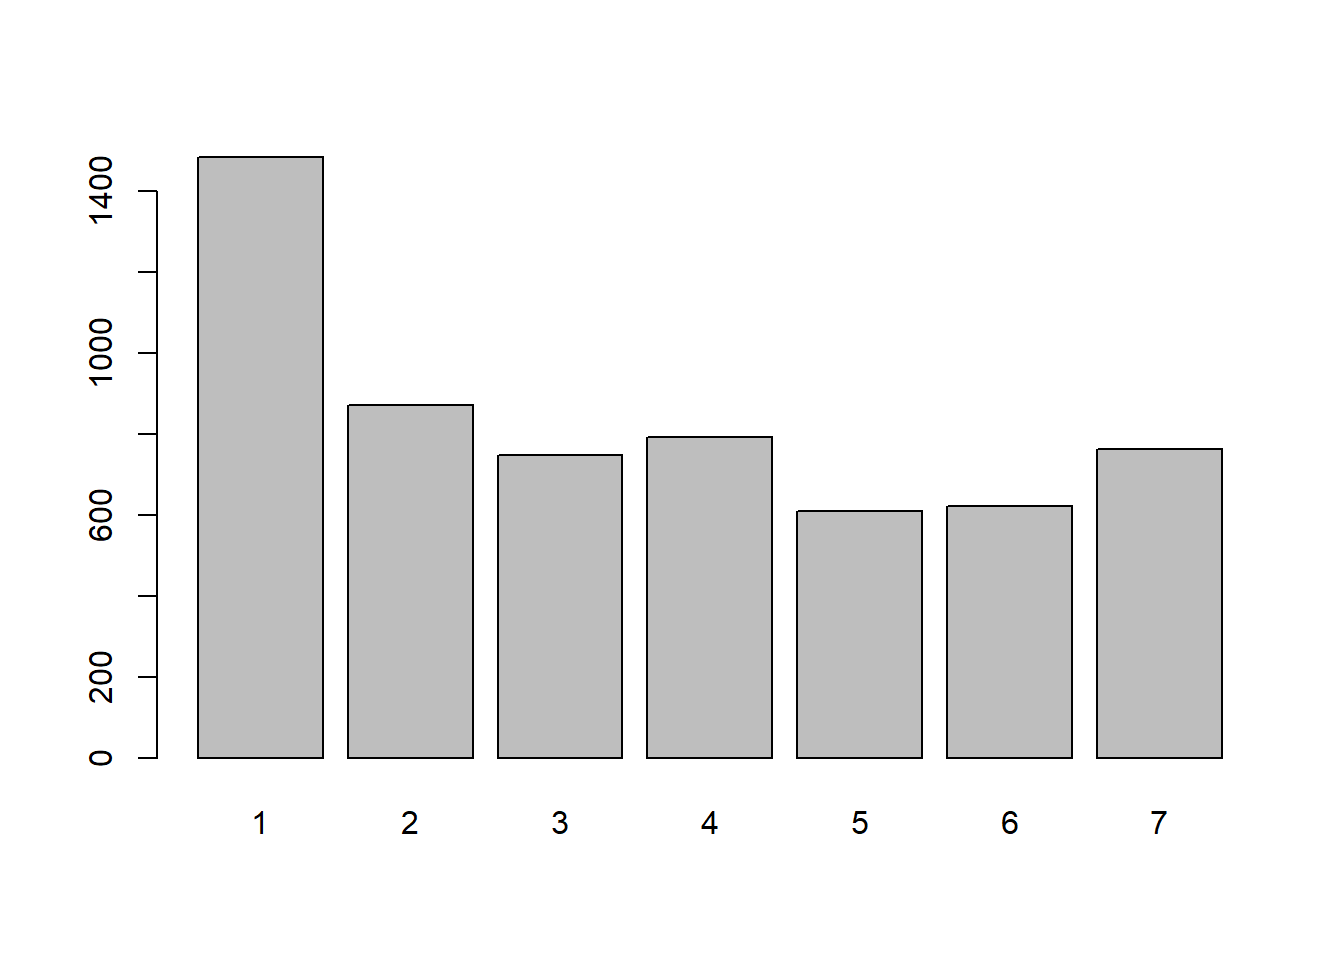
\includegraphics{psc-253-manual_files/figure-latex/unnamed-chunk-34-2.pdf}

\begin{verbatim}
## nes$pid7 
##       Frequency  Percent Valid Percent
## 1          1485  25.1014         25.20
## 2           873  14.7566         14.82
## 3           747  12.6268         12.68
## 4           792  13.3874         13.44
## 5           610  10.3110         10.35
## 6           623  10.5308         10.57
## 7           762  12.8803         12.93
## NA's         24   0.4057              
## Total      5916 100.0000        100.00
\end{verbatim}

\hypertarget{troubleshooting-13}{%
\subsection{Troubleshooting}\label{troubleshooting-13}}

\begin{itemize}
\tightlist
\item
  Have not come across any problems yet.
\end{itemize}

\hypertarget{subset}{%
\section{Create a Subset of Data}\label{subset}}

\hypertarget{problem-16}{%
\subsection{Problem}\label{problem-16}}

You want to create a subset of your data based on some criteria.

\hypertarget{solution---basic}{%
\subsection{Solution - Basic}\label{solution---basic}}

\begin{enumerate}
\def\labelenumi{\arabic{enumi}.}
\tightlist
\item
  Provide a name for the subset of data you are creating.
\item
  Use \texttt{subset()}. The main arguments are the data object that is being subsetted, the criteria for determining which observations to include in the subset, and the selection of columns for inclusion in the new data object.
\item
  The criteria use relational logic such as \texttt{==}, \texttt{\textgreater{}}, \texttt{!=}, etc.
\item
  Follow the template below.
\end{enumerate}

\begin{Shaded}
\begin{Highlighting}[]
\NormalTok{newdata }\OtherTok{\textless{}{-}} \FunctionTok{subset}\NormalTok{(old\_data, criteria, }\AttributeTok{select =} \FunctionTok{c}\NormalTok{(list of columns))}
\end{Highlighting}
\end{Shaded}

Here we create a subset that only includes people who voted for Obama.

\begin{Shaded}
\begin{Highlighting}[]
\CommentTok{\# frequency of \textasciigrave{}obama\_vote\textasciigrave{} in full dataset}
\FunctionTok{freq}\NormalTok{(nes}\SpecialCharTok{$}\NormalTok{obama\_vote)}
\end{Highlighting}
\end{Shaded}

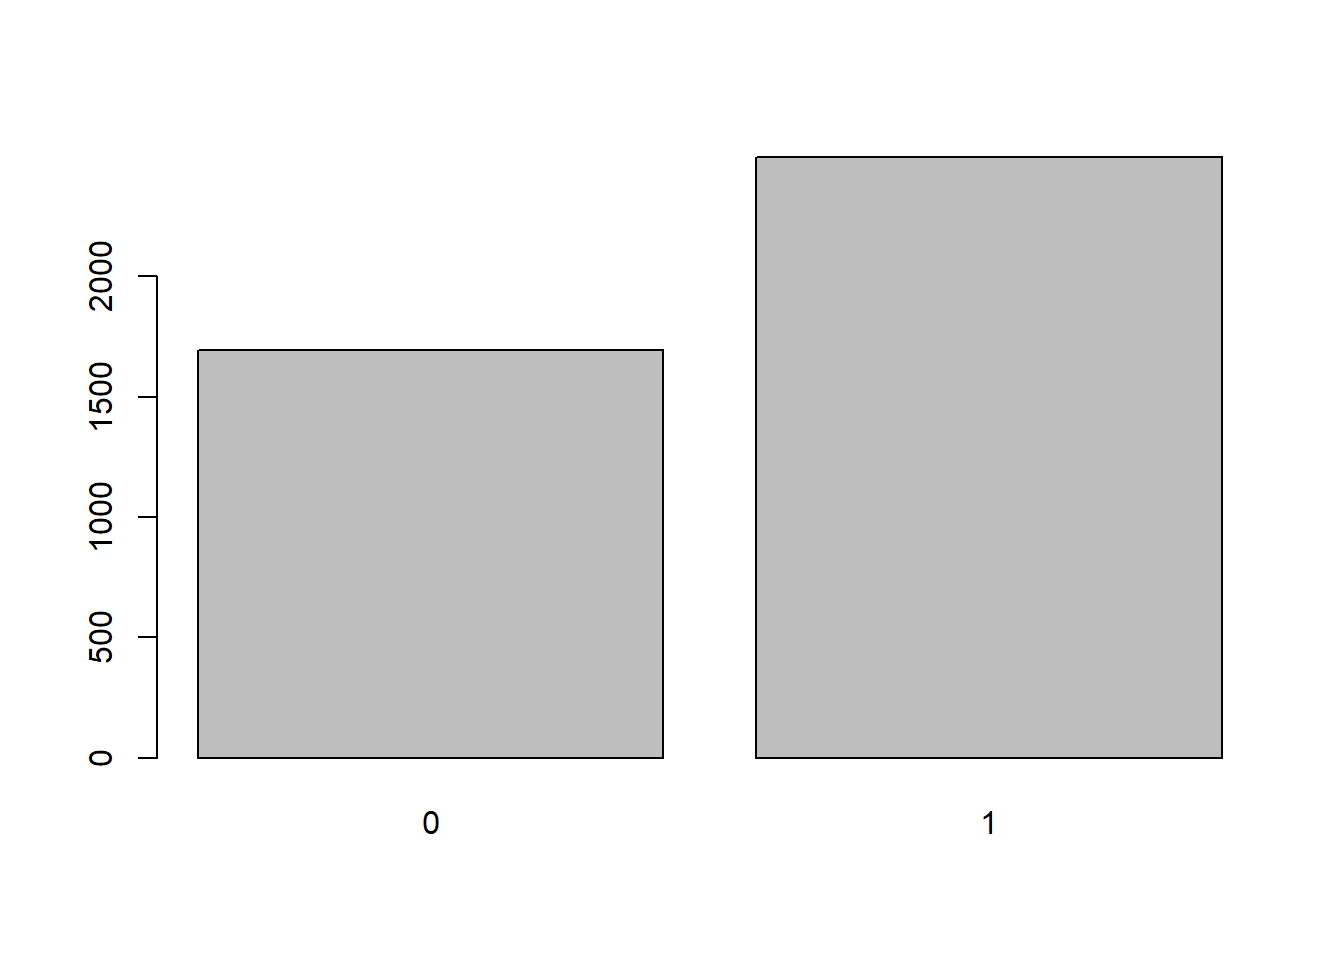
\includegraphics{psc-253-manual_files/figure-latex/unnamed-chunk-36-1.pdf}

\begin{verbatim}
## nes$obama_vote 
##       Frequency Percent Valid Percent
## 0          1692   28.60          40.4
## 1          2496   42.19          59.6
## NA's       1728   29.21              
## Total      5916  100.00         100.0
\end{verbatim}

\begin{Shaded}
\begin{Highlighting}[]
\CommentTok{\# create a subset of \textasciigrave{}nes\textasciigrave{} data that only includes Obama voters}
\NormalTok{ovoters }\OtherTok{\textless{}{-}} \FunctionTok{subset}\NormalTok{(nes, obama\_vote }\SpecialCharTok{==} \DecValTok{1}\NormalTok{)}

\CommentTok{\# frequency of a \textasciigrave{}obama\_vote\textasciigrave{} in subset}
\FunctionTok{freq}\NormalTok{(ovoters}\SpecialCharTok{$}\NormalTok{obama\_vote)}
\end{Highlighting}
\end{Shaded}

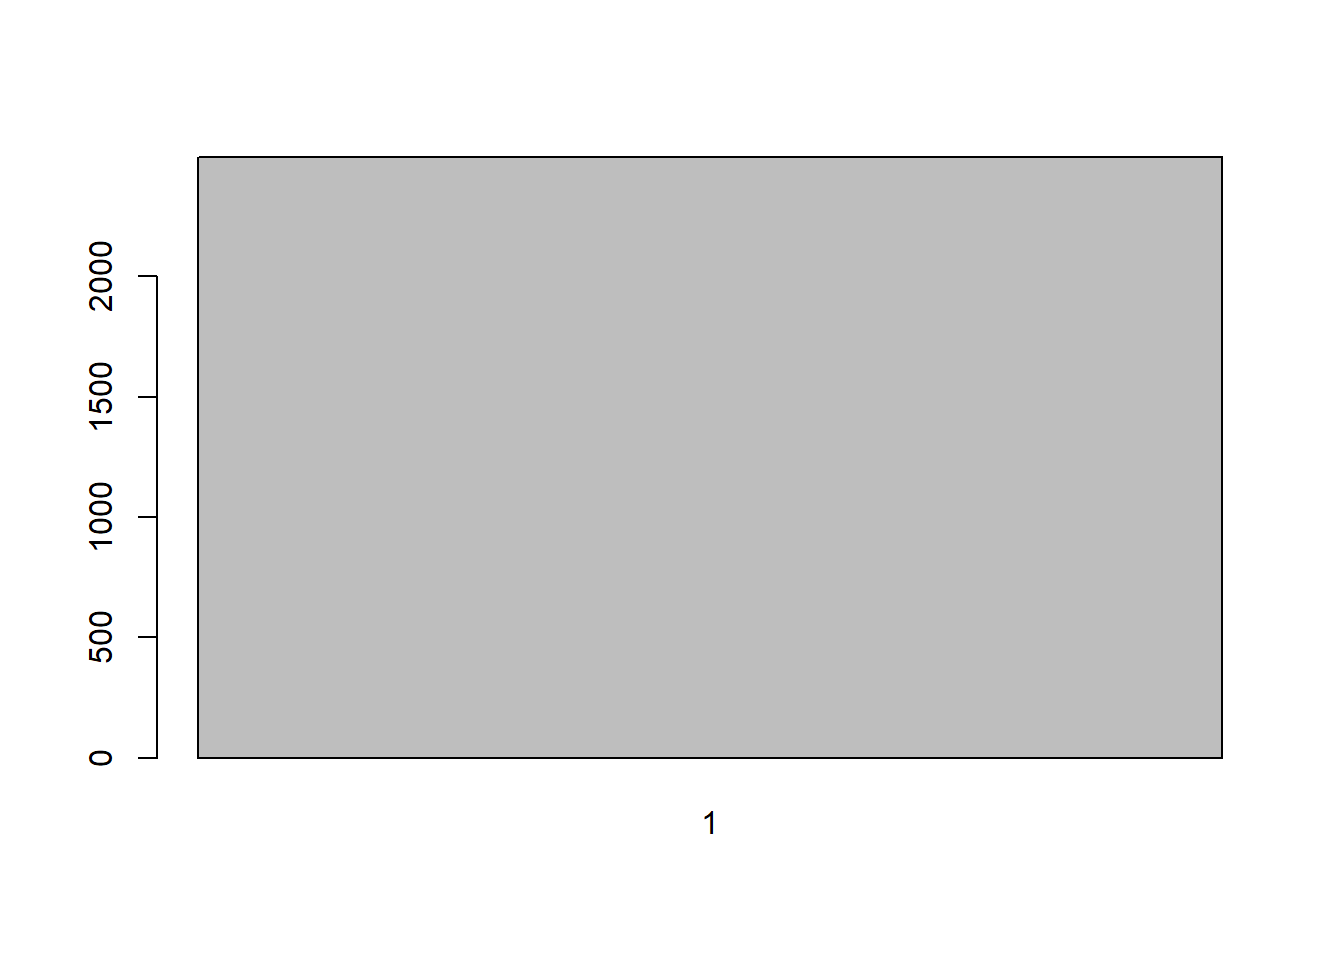
\includegraphics{psc-253-manual_files/figure-latex/unnamed-chunk-36-2.pdf}

\begin{verbatim}
## ovoters$obama_vote 
##       Frequency Percent
## 1          2496     100
## Total      2496     100
\end{verbatim}

\hypertarget{solution---tidyverse}{%
\subsection{Solution - Tidyverse}\label{solution---tidyverse}}

\begin{enumerate}
\def\labelenumi{\arabic{enumi}.}
\tightlist
\item
  Provide a name for the subset of data you are creating.
\item
  Assign the existing dataset to the new data object.
\item
  Use the pipe \texttt{\%\textgreater{}\%}.
\item
  Use \texttt{filter()}. The pipe inherits the dataset from the prior step, so the only argument is the criteria for the subset.
\item
  The criteria use relational logic such as \texttt{==}, \texttt{\textgreater{}}, \texttt{!=}, etc.
\item
  Follow the template below.
\end{enumerate}

\begin{Shaded}
\begin{Highlighting}[]
\NormalTok{newdata }\OtherTok{\textless{}{-}}\NormalTok{ old\_data }\SpecialCharTok{\%\textgreater{}\%}
  \FunctionTok{filter}\NormalTok{(criteria)}
\end{Highlighting}
\end{Shaded}

Here we create a subset that only includes people who voted for Obama.

\begin{Shaded}
\begin{Highlighting}[]
\CommentTok{\# frequency of \textasciigrave{}obama\_vote\textasciigrave{} in full dataset}
\FunctionTok{freq}\NormalTok{(nes}\SpecialCharTok{$}\NormalTok{obama\_vote)}
\end{Highlighting}
\end{Shaded}

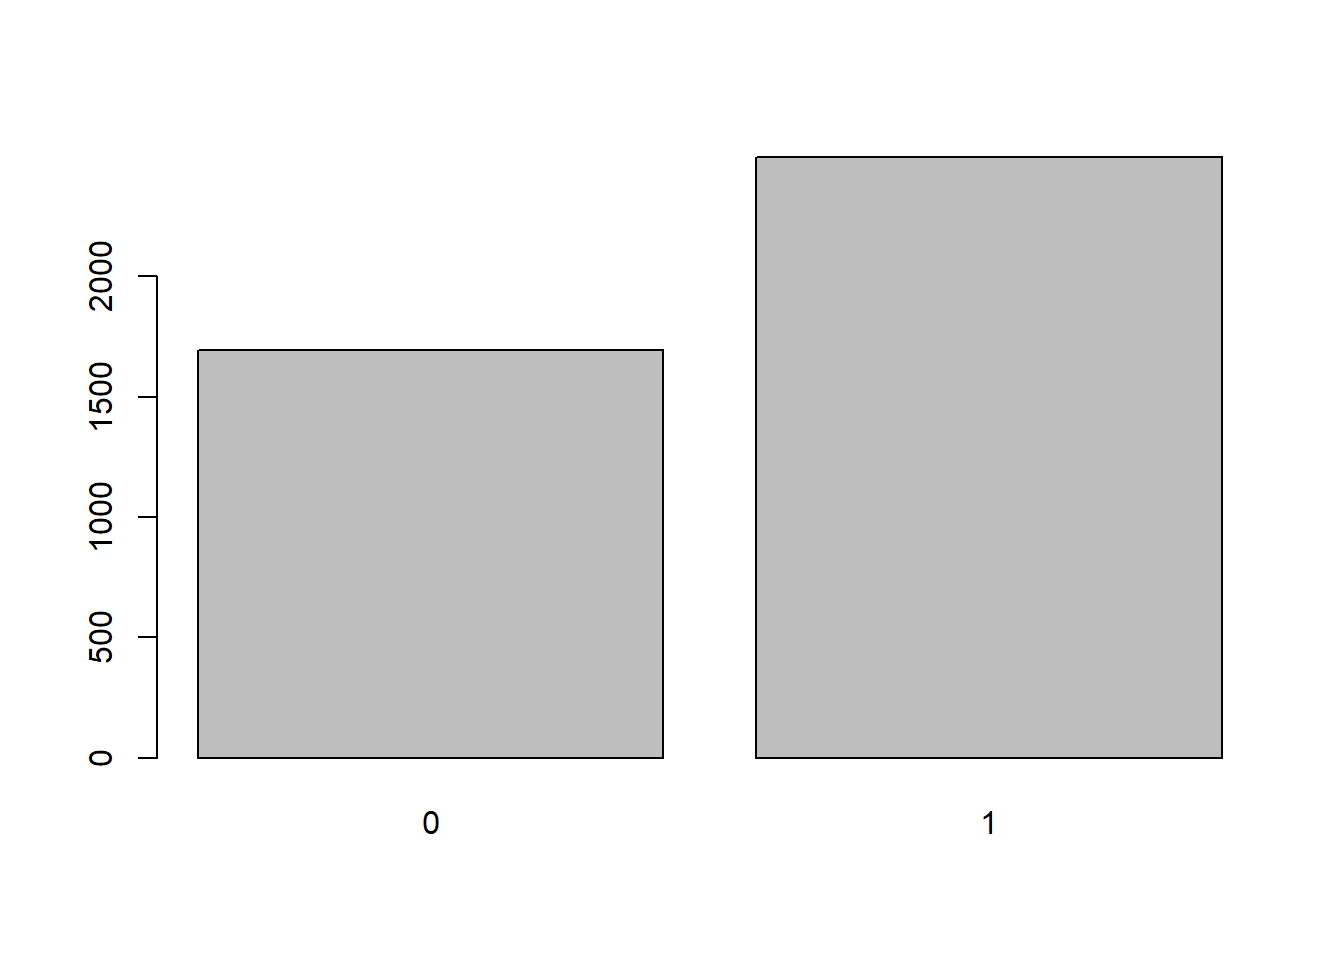
\includegraphics{psc-253-manual_files/figure-latex/unnamed-chunk-38-1.pdf}

\begin{verbatim}
## nes$obama_vote 
##       Frequency Percent Valid Percent
## 0          1692   28.60          40.4
## 1          2496   42.19          59.6
## NA's       1728   29.21              
## Total      5916  100.00         100.0
\end{verbatim}

\begin{Shaded}
\begin{Highlighting}[]
\CommentTok{\# create a subset of \textasciigrave{}nes\textasciigrave{} data that only includes Obama voters}
\NormalTok{obamites }\OtherTok{\textless{}{-}}\NormalTok{ nes }\SpecialCharTok{\%\textgreater{}\%}
  \FunctionTok{filter}\NormalTok{(obama\_vote }\SpecialCharTok{==} \DecValTok{1}\NormalTok{)}

\CommentTok{\# frequency of a \textasciigrave{}obama\_vote\textasciigrave{} in subset}
\FunctionTok{freq}\NormalTok{(obamites}\SpecialCharTok{$}\NormalTok{obama\_vote)}
\end{Highlighting}
\end{Shaded}

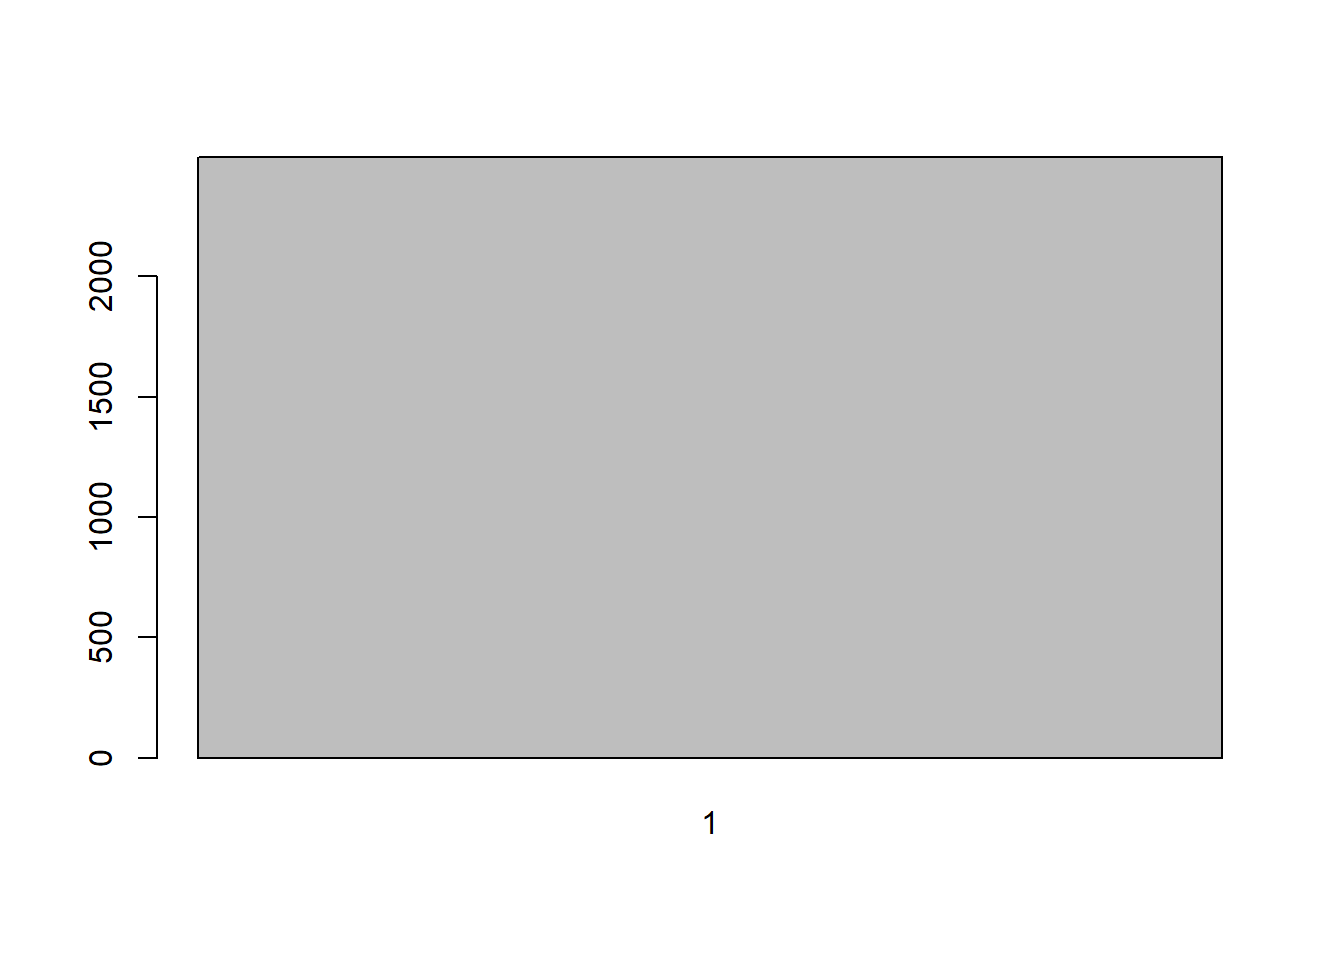
\includegraphics{psc-253-manual_files/figure-latex/unnamed-chunk-38-2.pdf}

\begin{verbatim}
## obamites$obama_vote 
##       Frequency Percent
## 1          2496     100
## Total      2496     100
\end{verbatim}

\hypertarget{troubleshooting-14}{%
\subsection{Troubleshooting}\label{troubleshooting-14}}

\begin{itemize}
\tightlist
\item
  Make sure that your subset is assigned to something.
\item
  The criteria is written as variable, logical operator, and value of the variable.
\item
  The values of categorical variables must be in quotation marks.
\end{itemize}

\hypertarget{sum}{%
\section{Summarize Data Using Means}\label{sum}}

\hypertarget{problem-17}{%
\subsection{Problem}\label{problem-17}}

You want to make a summary dataset that shows the mean of one variable for each value of some other variable.

\hypertarget{solution-16}{%
\subsection{Solution}\label{solution-16}}

\begin{enumerate}
\def\labelenumi{\arabic{enumi}.}
\tightlist
\item
  Assign the old data to a new data object.
\item
  Use the pipe \texttt{\%\textgreater{}\%} at the end of the line of code.
\item
  Use \texttt{group\_by()}. The argument is the variable that you want to use to find the means of some other variable.
\item
  Use the pipe \texttt{\%\textgreater{}\%} at the end of the line of code.
\item
  Use \texttt{summarise()}.
\item
  Create a name for the summary variable.
\item
  Set the summary variable as being equal to the mean of the variable that you want to take the mean of.
\end{enumerate}

\begin{Shaded}
\begin{Highlighting}[]
\NormalTok{newdata }\OtherTok{\textless{}{-}}\NormalTok{ old\_data }\SpecialCharTok{\%\textgreater{}\%}
  \FunctionTok{group\_by}\NormalTok{(group\_variable) }\SpecialCharTok{\%\textgreater{}\%}
  \FunctionTok{summarise}\NormalTok{(}\AttributeTok{summary\_variable =} \FunctionTok{mean}\NormalTok{(mean\_variable))}
\end{Highlighting}
\end{Shaded}

Here we calculate the mean feelings towards Obama, \texttt{obama\_therm}, by party identification, \texttt{pid\_x}.

\begin{Shaded}
\begin{Highlighting}[]
\CommentTok{\# assign old data to a new data object}
\NormalTok{partymeans }\OtherTok{\textless{}{-}}\NormalTok{ nes }\SpecialCharTok{\%\textgreater{}\%}
  
  \CommentTok{\# use group\_by() to group the data by pid\_x}
  \FunctionTok{group\_by}\NormalTok{(pid\_x) }\SpecialCharTok{\%\textgreater{}\%}
  
  \CommentTok{\# calculate the means of obama\_therm}
  \FunctionTok{summarise}\NormalTok{(}\AttributeTok{average =} \FunctionTok{wtd.mean}\NormalTok{(obama\_therm, }\AttributeTok{na.rm =}\NormalTok{ T,}
                               \AttributeTok{weights =}\NormalTok{ wt))}

\CommentTok{\# show the summary dataset}
\NormalTok{partymeans}
\end{Highlighting}
\end{Shaded}

\begin{verbatim}
## # A tibble: 8 x 2
##   pid_x  average
##   <fct>    <dbl>
## 1 StrDem    90.1
## 2 WkDem     74.2
## 3 IndDem    75.2
## 4 Ind       53.3
## 5 IndRep    32.8
## 6 WkRep     36.7
## 7 StrRep    17.6
## 8 <NA>      61.0
\end{verbatim}

\hypertarget{troubleshooting-15}{%
\subsection{Troubleshooting}\label{troubleshooting-15}}

\begin{itemize}
\tightlist
\item
  For survey data use \texttt{wtd.mean()}. Use \texttt{mean()} for non-survey data.
\end{itemize}

\hypertarget{missing}{%
\section{Label Missing Observations in a Dataset}\label{missing}}

Sometimes we will work with survey data that has observations with numeric codes that are not aligned with a response of interest. For example, the numeric code -9 might signify that a person did not actually answer the survey question. We want to label this particular observation as ``missing''.

\hypertarget{problem-18}{%
\subsection{Problem}\label{problem-18}}

You want to label missing observations.

\hypertarget{solution-17}{%
\subsection{Solution}\label{solution-17}}

  \bibliography{book.bib,packages.bib}

\end{document}
